
%%%%%%%%%%%%%%%%%%%%%%%%%%%%%%%%%%%%%%%%%%%%%%%%%%%%%%%%%%%%%%%%%%%%%
% PREAMBLE
%%%%%%%%%%%%%%%%%%%%%%%%%%%%%%%%%%%%%%%%%%%%%%%%%%%%%%%%%%%%%%%%%%%%%
%
% The following two commands will generate a PDF that follows all the requirements for submission
% and peer review.  Uncomment these commands to generate this output (and comment out the two lines below.)
%
% DOUBLE SPACE VERSION FOR SUBMISSION TO THE AMS
\documentclass[pdftex,12pt]{article}
\usepackage{ametsoc}
\linenumbers
%
% The following two commands will generate a single space, double column paper that closely
% matches an AMS journal page.  Uncomment these commands to generate this output (and comment
% out the two lines above. FOR AUTHOR USE ONLY. PAPERS SUBMITTED IN THIS FORMAT WILL BE RETURNED
% TO THE AUTHOR for submission with the correct formatting.
%
% TWO COLUMN JOURNAL PAGE LAYOUT FOR AUTHOR USE ONLY
%\documentclass[10pt]{article}
%\usepackage{ametsoc2col}
%

%%%%%
% JRL : Custom packages that I might need to remove!
\usepackage{rotfloat} % Rotated images
\usepackage{rotating} % Rotated images
\usepackage{subfig} % JRL; For multiple images in figures

%% JRL: user commands and packages here...
\def\mps{m\,s$^{-1}$}
\def\MW{\mbox{MesoWest}} %Avoid line breaks
\def\gpt{$\nabla \theta_{DT}$}
\def\degarc{$^{\circ}$} %For lat/lon, angle of wind etc
\def\degC{$^{\circ}$C} %For Celsius
\def\around{$\sim$}
\def\gt{\textgreater}
\def\lt{\textless}
\usepackage{array} % Tables of fixed columns
\newcolumntype{P}[1]{>{\raggedright\arraybackslash}p{#1}} % Tables of fixed columns
%%%%%

%%%%%%%%%%%%%%%%%%%%%%%%%%%%%%%%%%%%%%%%%%%%%%%%%%%%%%%%%%%%%%%%%%%%%
% ABSTRACT
%
% Enter your Abstract here
%%%%%%%%%%%%%%%%%%%%%%%%%%%%%%%%%%%%%%%%%%%%%%%%%%%%%%%%%%%%%%%%%%%%%
\newcommand{\myabstract}{A downslope windstorm on 1 December 2011 led to considerable damage along a narrow 50-km swath at the western base of the Wasatch Mountains in northern Utah. The strongest surface winds began suddenly at 0900\,UTC, primarily in the southern portion of the damage zone. Surface winds reached their peak intensity with gusts to 45\,\mps{} at \around 1600\,UTC, while the strongest winds shifted later to the northern end of the damage swath. The northward shift in strong surface winds relates to the rotation of synoptic-scale flow from northeasterly to easterly at crest level, controlled by an evolving anticyclonic Rossby-wave-breaking event. A rawinsonde released at \around 1100\,UTC in the midst of strong (\gt 35\,\mps) easterly surface wind intersected a rotor and sampled the strong inversion that surmounted it. 

The windstorm's evolution was examined further via Weather Research and Forecasting model simulations initialized from North American Mesoscale analyses \around 54\,h before the windstorm onset. The control model simulation captured core features of the event, including the spatial extent and timing of the strongest surface winds. However, the model developed stronger mountain-wave breaking in the lee of the Wasatch, a broader zone of strong surface winds, and a downstream rotor located farther west than observed. A second simulation, in which the nearby east--west-oriented Uinta mountains were reduced in elevation, developed weaker easterly flow across the Wasatch during the early stages of the event. This result suggests that the Uinta Mountains  block and steer the initial northeasterly flow across the Wasatch.}

%A rawinsonde released at \around 1100\,UTC in the midst of strong (\gt 35\,\mps) easterly surface winds initially travelled horizontally before ascending rapidly within a downstream rotor. The sonde subsequently intersected a strong inversion at the top of the rotor due to dry air descending sharply from above crest level.

%
\begin{document}
%
%%%%%%%%%%%%%%%%%%%%%%%%%%%%%%%%%%%%%%%%%%%%%%%%%%%%%%%%%%%%%%%%%%%%%
% TITLE
%
% Enter your TITLE here
%%%%%%%%%%%%%%%%%%%%%%%%%%%%%%%%%%%%%%%%%%%%%%%%%%%%%%%%%%%%%%%%%%%%%
\title{\textbf{\large{Analysis of the 1 December 2011 Wasatch downslope windstorm}}}



%
% Author names, with corresponding author information. 
% [Update and move the \thanks{...} block as appropriate.]
%
\author{\textsc{John Lawson}
    			\thanks{\textit{Corresponding author address:} 
				John Lawson, Department of Geological and Atmospheric Science, 
				Iowa State University, Ames, IA 50011. 
				\newline{E-mail: john.rob.lawson@googlemail.com}}\quad\textsc{and John Horel}\\
\textit{\footnotesize{Department of Atmospheric Science, University of Utah, Salt Lake City, Utah, United States of America.}}
}
%
% Formatting done here...Authors should skip over this.  See above for abstract.
\ifthenelse{\boolean{dc}}
{
\twocolumn[
\begin{@twocolumnfalse}
\amstitle

% Start Abstract (Enter your Abstract above.  Do not enter any text here)
\begin{center}
\begin{minipage}{13.0cm}
\begin{abstract}
	\myabstract
	\newline
	\begin{center}
		\rule{38mm}{0.2mm}
	\end{center}
\end{abstract}
\end{minipage}
\end{center}
\end{@twocolumnfalse}
]
}
{
\amstitle
\begin{abstract}
\myabstract
\end{abstract}
\newpage
}
%%%%%%%%%%%%%%%%%%%%%%%%%%%%%%%%%%%%%%%%%%%%%%%%%%%%%%%%%%%%%%%%%%%%%
% MAIN BODY OF PAPER
%%%%%%%%%%%%%%%%%%%%%%%%%%%%%%%%%%%%%%%%%%%%%%%%%%%%%%%%%%%%%%%%%%%%%
\section{Introduction}
Downslope windstorms arise when a layer of air is sandwiched between a terrain barrier and a strongly-stable layer aloft, while being forced over the barrier \citep{Markowski2010}. Due to the damage often associated with downslope windstorms, they have obtained local names in areas experiencing them frequently, including the f\"ohn, bora, chinook, zonda, Santa Ana, Wasatch, and Washoe Zephyr \citep{Whiteman2000,Richner2013}. As discussed by \citet{Richner2013}, the general synoptic features associated with localized downslope windstorms are well understood and reasonably well predicted. 

The Wasatch windstorm of 1 December 2011 caused over \$75 million damage in a narrow swath, roughly 3--5\,km wide and 50\,km long as delineated by the hatched rectangular box in Fig.~\ref{fig:wasatchmap}a along the Wasatch Front \citep{O'Donoghue2012}. The Wasatch Front describes the urban--suburban corridor paralleling the west slopes of the Wasatch Mountains.   Impacts of this storm, which was later declared a federal disaster, included: as many as 70,000 trees were uprooted or damaged; power was lost in many communities after over 22 transformers were damaged and 1.5\,km of power lines required maintenance; rail traffic was halted along the Wasatch Front; and Interstate 15 was closed to large vehicles after many were blown over on the freeway.

An anemometer sited by Union Pacific Railroad in Centerville, UT (UP028 in Fig.~\ref{fig:wasatchmap}b), along a stretch of rail line prone to high winds during downslope windstorms, recorded a maximum gust of 45\,\mps{} (102\,mph) at \around 1600\,UTC \footnote{Local time in Utah is 7\,h earlier than UTC during winter.} 1 December 2011 (Fig.~\ref{fig:cenwws}). Strong winds were not only observed along the Wasatch Front on this day, but also in other localized areas across the western United States; for example, southern California experienced one of its strongest Santa Ana events in recent years \citep{Welch2011}.

Forecasting the occurrence of downslope windstorms has long been recognized to require several critical ingredients \citep{Smith1985,Markowski2010}. Following \citet{Markowski2010}, the terrain barrier must first be: (1) quasi-two-dimensional so that air cannot simply flow around it, and (2) asymmetrical with a more gentle windward slope combined with a steep lee slope \citep{Miller1991-tf}. However, no single terrain characteristic is tied to strong-windstorm environments. Figure~\ref{fig:cenwws} depicts the steep lee-side profile along the Wasatch Front, near Centerville, UT. Here, the flat base of elevation 1280\,m above mean sea-level rises eastward towards the crest of the Wasatch mountains (2500--2750\,m in this region).

%As shown in Table~\ref{tab:slope}, there is no obvious dependence on the downstream valley-to-crest vertical distance. In addition, the lee-side slope gradient is variable; windstorms have been documented in the lee of crests that rise only 200--300\,m above the downstream valley \citep{Marriott1886,Mobbs2005,Decker2011}. 

Second, a sufficiently-strong cross-barrier wind (\gt 15\,\mps) must impinge on the barrier; a wind direction orthogonal to a two-dimensional barrier will maximize the cross-product of the crest orientation and wind direction, and hence mountain wave excitation in the same direction downstream. Third, the vertical profiles of temperature, moisture, and wind should be conducive to amplifying the development of mountain lee waves. This typically requires one or more of the following characteristics: (1) a strongly-stable layer upstream of and above the crest level \citep{Vosper2004}; (2) an environmental critical level above crest level, where the cross-wind component decreases to zero and/or reverses direction (e.g., \citealt{Wang1999-va}); (3) a wave-induced critical level \citep{Peltier1979}, where wave-breaking itself generates a wind reversal above crest level that is not found in upstream wind profiles; or (4) the synoptic environment should favor subsidence aloft, but not favor the development of a deep cold-air pool in the lee of the range that might inhibit penetration of strong winds to the surface \citep{Jiang2008}. 

National Weather Service (NWS) forecasts issued by the Salt Lake City Forecast Office for the 1 December 2011 Wasatch windstorm were ample for public and private contingency planning in terms of spatial and temporal accuracy, forecast lead time, and wind speed magnitude. The first Area Forecast Discussion (AFD) to mention a potential for strong winds along the Wasatch Front on 1 December was issued at 1712\,UTC 27 November (90\,h before the onset of the windstorm) and the matter was discussed in the subsequent Hazardous Weather Outlook (HWO). All further AFDs and HWOs issued by the Salt Lake City Forecast Office mentioned the chance for high winds, with increasing confidence as the event drew closer. The potential for high winds was cited in many AFDs to be based on: (1) the similarity between the developing synoptic situation and situations observed during prior major Wasatch windstorms, and (2) confidence in both the numerical model guidance from operational forecast models and a higher-resolution model run locally at the Forecast Office \footnote{Weather Research and Forecasting mesoscale model runs were made four times a day with boundary conditions based on the prior Global Forecast System model. The regional domain was 12\,km, and nested down to 4\,km across Utah. Each run produced hourly guidance through 60 forecast hours. This was the first major Wasatch windstorm where forecasters had access to high-resolution forecast guidance in their operational office environment (Randy Graham and Steve Rogowski, 2012, personal communication).}.

Planning for this study began the day before the windstorm, and was motivated by a number of factors: (1) operational numerical guidance and forecaster experience led to high confidence that a major downslope windstorm was possible; (2) verification of this forecast would lead to the first major downslope windstorm along the Wasatch Front in over a decade; (3) experimental high-resolution numerical forecasts run by the Salt Lake City National Weather Service Office were providing considerable specificity regarding the details of the impending windstorm; and (4) routine automated observations were already in place throughout the region such that additional observational assets available in the Department of Atmospheric Sciences could be used advantageously to mount a small field campaign to study the event (the equipment available has been described by \citealt{Lareau2013}). On 30 November, a University of Utah (UoU) team quickly drew up a research plan to collect additional observations the next day using surface weather stations, portable rawinsonde systems, and vehicle-mounted sensors. While a major downslope windstorm was deemed likely by forecasters, and supported by high-resolution deterministic model output, UoU team confidence was not particularly high regarding the specific details (timing, location, and intensity) of the high-resolution numerical guidance provided by the NWS.  

The resulting severity of the event, combined with the accuracy of the high-resolution model guidance, the apparent extended predictability, and an unprecedented data set for a Wasatch downslope windstorm, ultimately led to completion of this study. Our objectives are to examine the 1 December 2011 Wasatch downslope windstorm from several distinct perspectives: (1) relate briefly this event to previous downslope windstorms; (2) analyze the spatial and temporal evolution of the winds on the basis of local observations from conventional sources and those collected specifically during the small field campaign; (3) evaluate a high-resolution model simulation in terms of its ability to resolve the mesoscale and local features of the event; and (4) assess the impacts of the upstream Uinta Mountains that may deflect the flow traveling towards the Wasatch Mountains. \citet{Lawson2013a} provides additional details about this research.

\section{Data and Model Configuration}
\subsection{Observational data}

Surface observations of meteorological and other environmental parameters were obtained from the \MW{} archive \citep{Horel2002}. Reports from over 280 automated reporting stations were available within 80\,km (50\,mi) of Centerville, UT, the location of the strongest winds on 1 December 2011. There are substantive differences in the siting, equipment, and reporting characteristics of the automated observations available in \MW. Wind observations were manually evaluated to identify the time and intensity of the strongest observed winds.

An ad hoc UoU team of staff and students assembled during the morning of 30 November 2011 to determine where additional observations would help to document the expected windstorm. Decisions were made and implemented that afternoon to deploy three automated weather stations (locations shown in Fig.~\ref{fig:wasatchmap}b): (1) near Morgan, UT (\MW{} identifier UFD06), immediately east of the Wasatch Range and located roughly along the cross section shown in Fig.~\ref{fig:wasatchmap}a to monitor conditions upstream of the Wasatch; (2) east of Bountiful, UT (UFD05), \around 500\,m in elevation above the foot of the slope and as far up as it was practical to drive given the weather and mountain road conditions; and (3) Farmington (UFD04) in Farmington, UT, \around 1.5\,km west of the base of the Wasatch. Two mobile Graw rawinsonde systems were prepared for the next day: one to be sited where the portable automated weather station was deployed near Morgan, UT (upstream of the Wasatch Range); the other to be deployed as needed in the lee of the range based on how the conditions evolved. Two vehicles were also equipped with roof-mounted GPS, wind, temperature, humidity, and pressure sensors. However, one of the roof-mounted racks was destroyed early the next day in the high winds.

\subsection{Model setup}
Numerical simulations were performed with the Weather Research and Forecasting (WRF) model, version 3.4, using the Advanced Research WRF dynamical core. All runs comprised three nested domains of grid size 12, 4, and 1.3\,km (Fig.~\ref{fig:domains}), whose initial and boundary conditions (updated every 6\,h) were provided by North American Mesoscale (NAM) model analyses. The domains allowed two-way feedback; high-frequency waves were damped with sixth-order diffusion on the largest domain. Topography was interpolated from datasets at a resolution of 10\,min for the 12-km domain, and 30\,s for the 4- and 1.33-km domains, to the WRF-model grids. To avoid Courant-Friedrichs-Lewy criterion violation in regions of active mountain-wave breaking, vertical resolution was limited to 40 vertical levels. WRF output was interpolated onto a pressure-coordinate grid. Further details and parametrization options are listed in Table \ref{tab:param}.

\section{Results}
\subsection{Climatology}
Windstorms along the Wasatch Front (Fig.~\ref{fig:wasatchmap}) occur in climatologically-anomalous easterly flow at crest level \citep{Holland2002,Horel2002a}. Easterly windstorms \citep[e.g.,][]{Mass1985-at,Jones2002-la} are hence rarer than those that occur on lee slopes downwind of prevailing midlatitude westerly flows \citep[e.g.,][]{Lilly1972-ak,Zhong2008-rl}. As discussed by \citet{Holland2002}, few meteorological surface stations in the vicinity of the Wasatch Mountains are located in appropriate locations or have extensive enough records to develop climatologies of Wasatch windstorms. For example, the Salt Lake International Airport (KSLC in Fig.~\ref{fig:wasatchmap}) is too far west of the range and does not experience strong downslope winds during these events.

Following \citet{Holland2002}, observations from Hill Air Force Base (KHIF, Layton, UT in northern Davis County) are used to examine the occurrence of strong downslope winds between 1 October 1979 and 30 April 2012, the period for which European Centre for Medium-Range Weather Forecasts (ECMWF) Re-Analysis (ERA)-Interim data are available \citep{Dee2011}. KHIF has the longest and most reliable record of downslope windstorms of any observing site along the Wasatch Front. Due to its position 5\,km west of the Wasatch Front base, and near the exit of Weber Canyon, KHIF frequently experiences easterly winds associated with the Weber Canyon valley exit jet \citep{Chrust2013}, in addition to occasional downslope windstorms. \citet{Holland2002} found easterly wind gusts \gt 23\,\mps{} about 1.5 times per year during the entire observational period at the time (1953--1999), with more events observed in the earlier years than the later ones. Over time, there has been suburban development near KHIF, but not substantial enough to be responsible for the lower frequency of events in these later years. The strongest wind gust recorded at KHIF was 45\,\mps{} on 4 April 1983. \citet{Holland2002} derived composites of geopotential height on standard pressure levels for 79 strong easterly wind events using coarse-resolution (2.5\degarc{} latitude/longitude grid) National Centers for Environmental Prediction/National Center for Atmospheric Research reanalyses. Consistent with synoptic experience and forecasting practices at that time, the dominant composite signal described in that study was the development of a closed geopotential-height low on the 700-hPa surface, southwest of the Wasatch Mountains and centered near Las Vegas, NV. Receiving less attention in that study was the development to the north of the Wasatch Mountains of a composite geopotential-height ridge at 700\,hPa, which extended from coastal Washington state, curving through Montana, to Wyoming. This cyclone--anticyclone structure is consistent with the life-cycle 1 (LC1) type of Rossby-wave breaking \citep{Thorncroft1993}, i.e., anticyclonic Rossby-wave breaking (ARWB).

A more conservative definition for strong Wasatch windstorms than that applied by \citet{Holland2002} is used in this study. Observations at KHIF are taken automatically at hourly intervals, supplemented by occasional manual observations in between. A high wind event between October and April inclusive must satisfy the following criteria: (1) at least one KHIF observation with greater than 15\,\mps{} sustained winds from an easterly direction between 45\degarc{} and 135\degarc{}; and (2) ERA-Interim analyses must indicate a Rossby wave-breaking pattern (either anticylonic as described above, or cyclonic LC2 type with a trough or closed low tilting in the east- and poleward direction, \citealt{Thorncroft1993}). One strong easterly-wind event at KHIF met criterion (1), but not (2), and was ignored. In addition, multiday events were reduced to a single day if they were associated with the same upper-level wave-breaking event. We applied these criteria across the entire observational record available (1953--2012), as in \citet{Holland2002}. Constrained by the availability of ERA-Interim analyses from 1 January 1979 to present, and avoiding inclusion of only half a season, these criteria led to identification of 13 distinct downslope windstorms between 1 October 1979 and 30 April 2012 inclusive. Table~\ref{tab:dsws} shows their dates and sustained speeds and wind gusts.

The list of dates in Table~\ref{tab:dsws} and the time series of their occurrence during 1979--2012 (Fig.~\ref{fig:climoplot}) suggests that major downslope windstorms occurred once or twice every few years until 1999. Subsequently, no major downslope windstorm occurred until the 1 December 2011 event investigated here. The intermittence of Wasatch windstorms, particularly the lack of windstorms in the first decade of this century, raises the question whether their occurrence is determined by fewer Rossby-wave breaking events over western North America, or more directly, by fewer crest-level easterly wind periods during winter. \citet{Strong2008} developed an objective detection algorithm that generated a worldwide Rossby-wave-breaking climatology. Perhaps because their criteria allowed for weak and localized wave-breaking events, examination of their data as part of this study did not yield an obvious linkage of ARWB events to the occurrence of Wasatch windstorms. Figure~\ref{fig:climoplot} also shows the frequency of easterly (between 45\degarc{} and 135\degarc{}) crest-level (700\,hPa) winds over 10\,\mps{} during each winter season (October--April inclusive) from the ERA Interim Reanalyses. Since crest-level strong-easterly-wind periods do occur in the years that downslope windstorms were absent, the seasonal frequency of easterly winds is not a good predictor for the rare occurrences of downslope windstorms within those seasons. Hence, we can offer no definitive explanation for the absence of major Wasatch downslope windstorms during the 2000--2010 period.

In our set of 13 major windstorms (Table~\ref{tab:dsws}), the hour of peak wind at KHIF varies from 0700\,UTC to 1800\,UTC. In general, the peak in widespread downslope winds along the Wasatch Front tend to occur near sunrise (\around 1200\,UTC), since the dynamical forcing associated with the downslope winds is in phase at that time with the thermally forced Weber Canyon exit jet (\citealt{Chrust2013}). Hence, similar to \citet{Holland2002}, we show in Fig.~\ref{fig:700comp} composites of 700-hPa geopotential height, assuming that the peak downslope wind occurs near 1200\,UTC, and then composite conditions from 12\,h earlier (0000\,UTC) to 6\,h after (1800\,UTC). Southeastward progression of the tighter geopotential-height gradient associated with the breaking anticyclonic wave (e.g.,  Fig.~\ref{fig:700comp}b) marks the ARWB event, while the associated closed low deepens from 0000 to 1200\,UTC followed by filling. The strongest easterly gradient winds across the Wasatch Front are at 1200\,UTC.

When we compare the windstorm of 1 December 2011 to this climatological composite and to previous peak wind observations, we find it to be consistent with the upper-level signature of ARWB. It is also not only one of the strongest on record, but also the first in over ten years to match our criteria. In the next two subsections, we present observational and modeling data, respectively, to address why this was such a rare and damaging event.

\subsection{1 December 2011 windstorm}
Figure~\ref{fig:geopot4panel} summarizes the synoptic evolution of the ARWB event on 1 December 2011 in ERA-Interim geopotential height and wind data on the 700-hPa surface.  A small southwest-moving wave in the height field, accompanied by a jet maximum, moves faster than the mean flow towards the base of the trough between 0000 and 1200\,UTC. The transport of cyclonic vorticity into the trough axis may contribute to the deepening of the closed low over the Nevada--Utah–-Arizona borders: 700-hPa heights drop 60\,m between 0000 and 0600\,UTC, and fall another 30\,m between 0600 and 1200\,UTC. Lower-tropospheric cyclogenesis is often seen with LC1 baroclinic waves \citep{Thorncroft1993}. The closed-low center does not move far while its central height falls and the anticyclonic ridge breaks to the north. This clockwise pivoting of the breaking wave, and its slow southeastward progression, sustained a belt of 25\,\mps{} easterly winds on the northwestern quadrant of the low-height center. By 1200\,UTC, the crest of the Wasatch Front (at \around 700\,hPa) lies within this belt of strong easterly flow.

A longitude--pressure cross-section of zonal wind and potential temperature, taken on a west--east slice at 1200\,UTC through ERA-Interim data, indicates a low-level easterly jet surmounted by a statically-stable layer to the east of the Wasatch Front (not shown). Farther aloft, cross-barrier flow reverses with height. As mentioned in section 1, both this elevated stable layer and the flow reversal are conducive to initiation and amplification of mountain waves.

The first northward mobile transect along the Wasatch Front between 0915 and 1015\,UTC captured the sudden onset of the strongest winds (Fig.~\ref{fig:mobmes}). Departing from the UoU campus, strong easterly winds were first encountered south of Centerville (UP028) with the peak winds found near Centerville. Strong easterly winds were also observed at the western mouth of the Weber River Canyon while speeds dropped off substantially farther east up the canyon. Union Pacific Railroad halted all train traffic at the eastern mouth of Weber Canyon, the end of the mobile-sensor transects in Fig.~\ref{fig:mobmes}. Temperature and pressure mobile observations indicated near-uniform potential temperature at the base of the Wasatch Front; lower potential temperatures in the Weber River Canyon reflected the contribution of thermally-driven canyon flows to wind speed in this area (not shown). A 50-m tower located at the mouth of Weber River Canyon \citep{Chrust2013} sampled winds at 3, 10, 30, and 50\,m above ground level. Mean wind speeds generally increase with sensor height during the period of strongest winds (1100--1900\,UTC, not shown). However, due to the turbulent nature of the combined exit and downslope flows, peak winds are roughly equivalent in the 10--50\,m range; notably, 3-m wind gusts are occasionally as strong as those much farther aloft.

Figure~\ref{fig:ob_ts}a shows the time series of surface winds at KHIF on 1 December 2011 with most observations reported at hourly intervals. The strongest downslope winds were observed at this location during 1500--1800\,UTC, preceded by a brief period of strong winds at 1200\,UTC. Wind speed and direction at UFD04, a temporary station in Farmington, UT, located 1.5\,km from the base of the Wasatch, captures the onset and cessation of the downslope windstorm at 0900 and 1900\,UTC, respectively (Figure~\ref{fig:ob_ts}b). Peak intensity in winds at this location occurred \around 1500--1600\,UTC. These two stations (KHIF and UFD04) are representative of the windstorm's characteristics along the foothills, including the time of peak winds occurring later farther north along the Wasatch Front. In contrast to the sudden onset and cessation of downslope winds in the valley, winds at the crest of the Wasatch as measured at Ogden Peak (OGP, Fig.~\ref{fig:ob_ts}c) show a persistent easterly flow with winds increasing in intensity until late afternoon.

%A snapshot of the spatial variability in wind, temperature, and moisture at 1200\,UTC 1 December is shown in Fig.~\ref{fig:mesowest12z}. This display from data archived in MesoWest shows wind barbs and values of wind gusts at all available stations, as well as wind speed, direction, gusts, temperature, and dewpoint temperature at selected stations, which will be referred to here by their MesoWest station identifiers. The core location for the windstorm at this time is in the Farmington (UFD04) and Centerville (CEN) areas. In the Weber River Valley upstream (east) of the Wasatch Mountains, wind is light near the surface (Morgan, UFD06) and some flow channeling is evident near the exit of the the Weber River Canyon (Power Plant, PWR). Crest-level winds at OGP are quite strong, with slightly lower winds on the lee slope of the range (Bountiful Bench, UFD05). Westerly winds associated with rotor return flows are measured in some locations (UTLGP) while the prevailing strong northerly synoptic-scale flow is evident over the Great Salt Lake far away from the Wasatch range (Hat Island, HATUT). Winds are much lighter at KSLC slightly south of the domain plotted in Fig.~\ref{fig:mesowest12z}. Bursts of strong winds leading to uprooted trees were observed beginning at 1100\,UTC in northeastern portions of Salt Lake City (e.g., the University of Utah campus) where the terrain is favorable for downslope flow from the northeast (not shown). Dry-bulb temperatures are in the 1--4\degC{} range in most valley locations, and dewpoint temperatures are low (-7 to -12\degC). Over the next 6\,h, dry-bulb and dewpoint temperatures dropped as a result of the continued push of colder, drier air into the region (not shown).


%***REMOVE THIS SECTION? THE FIGURE?*** [An additional asset available to examine the vertical structure of the near-surface flows during this windstorm was a 50-m tower located at the mouth of Weber River Canyon \citep{Chrust2013}. This tower was installed to evaluate the wind energy potential from the frequent persistent nocturnal thermally-driven flows found at this valley exit-jet location. As shown in Fig.~\ref{fig:tower}, sensors at 3, 10, 30, and 50\,m indicate that mean wind speeds generally increase with sensor height during the period of strongest winds (1100--1900\,UTC). However, due to the turbulent nature of the combined exit and downslope flows, peak winds are roughly equivalent in the 10--50\,m range; notably, 3-m wind gusts are occasionally as strong as those much farther aloft.]

Vertical profiles of wind, temperature, and moisture, collected by rawinsondes launched twice-daily at KSLC during prior windstorms, have exhibited primarily the prevailing synoptic flow combined with complex downstream effects of the flow over the Wasatch Range. Figure~\ref{fig:kslcWRF} shows the KSLC sounding launched at \around 1100\,UTC with a nominal observation time of 1200\,UTC. The profile exhibits features typically observed at KSLC during a Wasatch windstorm: (1) no indication of downslope winds near the surface (i.e., weak low-level southerly drainage flow down the Salt Lake Valley towards the Great Salt Lake); (2) strong easterly winds below and extending above crest level (700\,hPa); (3) easterly winds weakening aloft with limited cross-barrier flow at 500\,hPa; (4) little moisture evident in the profile; (5) a small surface-based inversion with a well-mixed layer extending upwards to \around 750\,hPa; (6) evidence of strong turbulence between 750 and 700\,hPa with superadiabatic lapse rates; and (7) a capping inversion layer near crest (\around 690\,hPa) with an adiabatic layer above that level to 650 hPa.

The UoU team planned to launch rawinsondes upstream and downstream of the Wasatch at roughly the same time as the nearby NWS launch at KSLC (\around 1100\,UTC), and then to continue operations as conditions warranted. These additional launches were intended to describe the flows upstream and immediately downstream of the terrain where the strongest winds were expected. Upstream launches near Morgan, UT were made at the nominal observation times of 1200, 1500, and 1800\,UTC (i.e., balloons released at 1100, 1400, and 1700\,UTC, respectively). Since short-period communication failures between the radio base station and the 1200 and 1500\,UTC sondes near Morgan created small data gaps of 25--75\,hPa in depth, the 1800\,UTC profile is shown in Fig.~\ref{fig:sound}a. The automated algorithms provided by the rawinsonde manufacturer tend to smooth excessively the wind observations, hence the following figures use raw, unsmoothed wind data. Upstream of the Wasatch Range, the lowest 750\,m is well-mixed and nearly adiabatic, below a string of stable layers up to 5\,km. A particularly strong inversion is evident at \around 3250\,m, an elevation roughly 500\,m above the crest of the Wasatch in this area, which caps a layer with higher relative humidity and the strongest easterly winds (\around 30\,\mps) observed at this time. Above the highest inversion, winds are substantively weaker, and relative humidity is lower. Notably, easterly winds are observed throughout the profile below 5000\,m.

A day previously, the UoU team selected a park in Centerville, UT for a lee-side rawinsonde launch. Fortuitously, its position was within the core of strongest wind observed during the event, located immediately upwind (\around 200\,m) of the UDOT tower (CEN) and Union Pacific Railroad tower (UP028), themselves immediately west of the Interstate 15 freeway (see Fig.~\ref{fig:cenwws}). Sound-barrier walls east of the freeway bracket the park on its north and south edges and contributed to channeling of the flow. Several trucks tipped over as they passed northward from the protection of the sound barrier into the unprotected zone on the freeway, as well as on the adjacent frontage road. It was under these extremely harsh conditions that the UoU team successfully launched a rawinsonde at 1100\,UTC at the park. The balloon initially travelled nearly horizontally towards the freeway, before gaining altitude and clearing trees located at the edge of the frontage road. Vertical profiles of potential temperature, relative humidity, and wind speed and direction from the 1200\,UTC Centerville sounding are shown in Fig.~\ref{fig:sound}b. Two small communication gaps occurred during the ascent, one at 3050--3200\,m, and another at 3400--3500\,m. The immediate surface layer (lowest 50--60\,m) is characterized by lower potential temperature and horizontal winds approaching 40\,\mps, consistent with the nearby surface wind gust observations of \around 36\,\mps{} at UP028 at this time. Following \citet{Armi2011}, this layer is referred to as the ``downslope underflow''.

A sharp inversion (5.7\,\degC{} increase in \around 3.5\,hPa) at 3300\,m caps a turbulent layer containing adiabatic, superadiabatic, and weakly stable sublayers between 1700\,m and 3300\,m. Relative humidity increases to 90\% through this depth and falls sharply through the inversion. Winds again increase to over 30\,\mps{} in the inversion layer, and rotate above the inversion to sharply-reduced cross-barrier flow above 3750\,m. This rotation is not evident upstream near Morgan, and may therefore be self-induced. The sharp inversion is consistent with flow separation as the air crosses the Wasatch; the downslope underflow descends steeply along the slope, while another strong easterly current flows outward near crest level (\around 3300\,m). All three sondes upstream of the Wasatch Range detected the strongest winds (25--30\,\mps) at 3100--3200\,m, consistent with the strong crest-level winds observed near the inversion layer above Centerville.

Figure~\ref{fig:ascent} contrasts the ascent rates at \around 1--2-s intervals experienced by the Morgan and Centerville rawinsondes. The ascent rate near Morgan, averaged from surface to 3300\,m, is 4.8\,\mps, which is roughly what would be expected given the amount of helium used in the balloon (e.g., the 1200 and 1500\,UTC sondes had average ascent rates of 4.5 and 5.3\,\mps, respectively). The Centerville rawinsonde, using a similar volume of helium, experienced vastly different conditions from that near Morgan. Consistent with visual tracking of the Centerville sonde until lost in the dark, the buoyancy imparted by the helium was initially negated by descending motions, resulting in a near-horizontal trajectory. Then, the rawinsonde ascended at increasingly rapid rates approaching 25\,\mps{} through the superadiabatic layer. Vertical speeds then decreased up to 2900\,m. The balloon made no headway vertically through the sharp inversion, and at times descended in that layer, which led to a large number of observations in this vicinity. Once clear of this layer, the balloon ascended at an average rate of 4.6\,\mps. Subtracting this mean ascent rate from the observed rate yields a crude estimate of peak vertical velocities $O$(20\,\mps) upwards and $O$(7.5\,\mps) downwards.

The violent ascent and descent of the balloon is consistent with visual evidence after sunrise of rotors (low-level vortices with horizontal axes parallel to the ridgeline in the lee of mountain range; \citealt{Doyle2002}). Satellite images and photos indicate an upstream cloud deck over the Wasatch evaporating in the air descending down the lee slope with distinctive rotor clouds evident to the west of the base of the slope (not shown). The quasi-uniform horizontal distance from the crest to the location of the rotor clouds is \around 10\,km (3--5\,km from the base of the mountains). The superadiabatic lapse rate in the layer 2000--2500\,m may result from the formation of rotor clouds and then subsequent evaporative cooling of the air when the clouds dissipate. Aircraft, dropsonde, and lidar observations from the Terrain-Induced Rotor Experiment (T-REX) provide more comprehensive depictions of the turbulence and rotors present in the lee of the Sierra Mountains during downslope windstorms \citep{Armi2011,Kuhnlein2013-gt}. For example, aircraft and lidar observations during T-REX detected vertical velocities greater than 10--15\,\mps{} in the ascending air beneath rotor clouds.


\subsection{Control simulation}
The ability of a numerical simulation to capture the core features observed during this windstorm is now examined. A numerical simulation, referred to as the Control simulation, was performed with the WRF model initialized from the NAM-model analysis at 0600\,UTC 29 November 2011, and forced thereafter on the outermost boundary by NAM analyses updated every 6\,h.  The Control simulation is initialized far enough in advance for mesoscale circulations to develop freely, and continues for 72\,h to encompass the entire downslope windstorm event. The simulated 700-hPa geopotential height fields for 0000--1800\,UTC 1 December (42--60\,h into the simulation) are shown in Fig.~\ref{fig:NAM-C_700}, taken from the largest (12-km) WRF domain. The model captures the synoptic-scale structure of this ARWB event, with a ridge developing and extending southeastward from northern Idaho into Wyoming, while the cut-off low becomes centered near the southern tip of Nevada. Relative to the 700-hPa circulation depicted in the ERA-Interim reanalyses, values of geopotential height simulated by the model are elevated by \around 60\,m everywhere, but the modeled height gradients are similar to those analyzed, particularly in the vicinity of the Wasatch Front. However, the model simulation is slower in its development of the ARWB event, with the cut-off low-height center deepening until 1800\,UTC.

Observed surface wind speeds near the Wasatch Front at 1200\,UTC and 2100\,UTC are superimposed on the surface wind fields simulated by the model in Fig.~\ref{fig:verif}. The simulated winds are comparable to those observed near the base of the lee slopes of the Wasatch Mountains at 1200\,UTC, including the localized maximum near Centerville. By later in the day (2100\,UTC), the model has shifted the strongest winds farther north, but the simulated winds appear too strong compared to observations. The winds along the crest in the model are lower than those observed; for example, simulated wind speeds were 10--15\,\mps, while the winds observed at OGP and other crest-level stations at Snowbasin Ski Resort (not shown) were greater than 20\,\mps{} (see also Fig.~\ref{fig:ob_ts}c). As will be shown in greater detail later, the model tends to accelerate the flow down the slopes of the Wasatch Mountains more strongly than is likely taking place. The WRF model develops rotors and trapped waves, and these phenomena appear in the valley surface winds at 2100\,UTC as bands of increased and decreased winds in bands oriented parallel to the upstream terrain. In this 1.3-km domain simulation, strong winds do not extend out over the Great Salt Lake, whereas operational NWS 4-km WRF model forecasts (not shown) suggested a westward extension of 25--30\,\mps{} gusts as far west as Antelope Island (labelled AI in Fig.~\ref{fig:verif}).

The time evolution of wind speed and direction during the simulated downslope windstorm is now related in Fig.~\ref{fig:glove_ts} to that observed at Farmington (UFD04)  (previously shown in Fig.~\ref{fig:ob_ts}b). The Control simulation shows remarkable agreement with the observations regarding the timing and general evolution of the intensity of the surface winds. However, the simulated windstorm continues for \around 2\,h longer than that observed.

Figure~\ref{fig:kslcWRF} compares the vertical profiles of temperature, moisture, and wind at KSLC at 1200\,UTC from the Control simulation to the observed sounding. The model captures the basic vertical structure, but the simulated vertical profiles differ from those observed in several key respects: (1) surface westerly return flow rather than decoupled down-valley winds; (2) peak easterly flow near the base of a stable layer at 775\,hPa relative to that observed near 700\,hPa; (3) deep well-mixed layer between 750--550 hPa with near-zero cross-barrier flow at 600\,hPa, and more stable conditions and weak cross-barrier flow above \around 475\,hPa; and (4) generally lower dewpoint temperature throughout the troposphere.

To further evaluate the control simulation, we now present cross-sections of potential temperature and horizontal wind from the control simulation. The first cross-section lies along the southwest--northeast (A--B) transect shown in Fig.~\ref{fig:wasatchmap}, starting from the Great Salt Lake, through Centerville and terminating near Lyman, WY (Fig.~\ref{fig:ppxswu}). The wind components from the WRF model are rotated 20\degarc{} counterclockwise to create plane-parallel winds at all levels. Note that the terrain height is lower in the model than that observed: as a result of smoothing, the model's Wasatch Range is \around 250\,m lower than the actual terrain.

In the top panel of Fig.~\ref{fig:ppxswu}, at 1200\,UTC, 20\,\mps{} flow from the northeast (right to left in the figure) approaches the Wasatch Front, and then plunges sharply into the valley as a downslope windstorm. Note how the colder air (lower potential temperature) pools in the upstream valley, effectively creating an unobstructed horizontal pathway for the low-level easterly jet. Downstream of the Wasatch crest, strong winds continue for more than 10\,km along the valley floor before forming a rotor. Under this first rotor, \mbox{5--10\,\mps{}} westerly winds oppose the windstorm easterlies. The area of strong surface winds is broader than observed, i.e., observations suggest the rotor clouds and return flow begin roughly 10\,km from the crest, while the model shifts that farther west. In the bottom panel, at 2100\,UTC, the upstream stable layer has intensified as a result of both terresterial heating and continued cold advection in the planetary boundary layer at \around 3000\,m. This enhances the formation of mountain waves above the upstream terrain. The formation of rotors at this time occurs closer to the crest, though it is important to note that these images are merely snapshots; the locations of the non-linear internal gravity waves shift with time as a result of dynamical and turbulent processes (e.g., \citealt{Hertenstein2009}).

As evident in the Skew-T diagram for KSLC (Fig.~\ref{fig:kslcWRF}), the model's strongest easterly winds tend to be at a lower height over the terrain than observed. This may explain the model's tendency to confine flow to follow the terrain slope more closely than observed, i.e., the elevated flow extending westward away from the crest is missing from the model. Note also that the simulated winds immediately above the Wasatch crest are weak (see also Fig.~\ref{fig:verif}), which contributes to flow descending at a steeper angle associated with the lee waves. The model also does not capture the strong capping inversion above the rotor observed near Centerville.

Cross-sections of vertical motion indicate ascent within the rotor at 1200\,UTC is on the order of 20--30\,\mps{} (not shown), which is broadly consistent with the ascent rate estimated from the Centerville rawinsonde at this time. However, the overall structure of the simulated downslope windstorm is too intense, relative to that inferred from the Centerville sounding and other observational evidence. The strong subsidence, 2-km plunging of the isentropes, and extreme drying in the lee of the mountains is not likely to have taken place during this event. The lee waves continue to amplify through the time of the later cross-section as evident by the isentropes in Fig.~\ref{fig:ppxswu} at 2100\,UTC.

Cross-sections perpendicular to the upstream flow (i.e., roughly north--south across a swath of lower terrain in Wyoming and extending into the Uinta mountains; C--D in Fig.~\ref{fig:wasatchmap}) are generated by rotating the wind components \around 5\degarc{} counterclockwise (Fig.~\ref{fig:normxswu}). At 1200\,UTC, the simulation generates a barrier-jet-like core of 15--20\,\mps{} easterly winds to the north of the Uinta mountains. By 2100\,UTC, the strong easterly flow has extended farther north, as the cut-off low reaches a position directly south of the Wasatch Front. These factors may help to explain the observed northward progression of strong winds along the Wasatch Front as a result of the more windstorm-favorable easterlies extending farther north later in the day. 

\subsection{Sensitivity to Uinta Mountains}
The Uinta Mountains are a substantial barrier and have the distinction of being the highest mountain range (a crest line above 3000\,m) in the contiguous United States oriented in the east--west direction. Their location south of the open expanses of western Wyoming may contribute to channeling easterly winds towards the Wasatch Mountains. To test the sensitivity of the windstorm's strength and occurrence to the upstream terrain, we now present results of a modeling experiment (referred to as the No-Uinta simulation) in which the Uinta Mountains are flattened. Following similar WRF-terrain modifications by \citet{West2011} and \citet{Alcott2013}, the impact of the Uinta Mountains on the 1 December 2011 Wasatch downslope windstorm is investigated by completing a simulation in which the terrain height of the Uintas above 2300\,m is lowered to that elevation on the 4- and 1.3-km domains (the Uintas remain unchanged on the 12-km domain to minimize discontinuities on the largest scales). This has two additional impacts: (1) the resultant void is replaced by a volume of standard-atmosphere air, and (2) soil temperatures are replaced with the deep-soil values in places where the upper soil layers have been removed. Due to the strong dynamical forcing of this event, these two changes are unlikely to greatly affect the simulation in comparison to the changes arising from the altered terrain. The use of two-way feedback between the nested domains implies that the Uintas' presence in the outer domain may still be felt to some extent on the inner domains, i.e., the impact of their removal may be underestimated here.  

Figure~\ref{fig:eastdiff} shows the zonal wind difference (No-Uinta minus Control) after reducing the height of the Uinta mountains. At 1200\,UTC, there is a strong increase--decrease dipole centered near Salt Lake City (marked by SLC). North of Salt Lake City, easterly winds have been markedly reduced by the removal of the Uinta Mountains (elevations of which are contoured in red). The decreased easterly flow north of the Uinta mountains' former position supports the hypothesis that the Uintas obstruct southward flow and create a barrier jet towards the northern Wasatch Front. Conversely, easterly winds have strengthened to the south of Salt Lake City, particularly around the city of Provo in the southern Wasatch Front. Without the Uintas, the northeasterly flow from Wyoming is unimpeded and plunges over the Wasatch farther south as a downslope windstorm in that region.

Later at 2100\,UTC---with or without the Uinta mountains---there are strong easterly winds in the northern Wasatch Front, confirming the importance of the orientation of large-scale midtropospheric winds; i.e., when the large-scale flow becomes more easterly, the impact of the blocking by the Uintas is lessened. The reduced elevation of the Uintas allows the windstorm to continue in the southern Wasatch Front at this time. Overall, an increased easterly component appears to initiate mountain waves more easily along the northern Wasatch Front. In contrast, the presence of the Uintas likely shields the southern Wasatch Front from damaging winds on many occasions. The time series of simulated surface wind at UFD04, with (green) and without (red) the Uintas, are shown in Fig.~\ref{fig:glove_ts}, and corroborates the sensitivity of valley wind speed to the orientation of the large-scale flow. Without the Uintas, the downslope easterly flow is weaker until the model's synoptic-scale flow becomes more easterly after 1500\,UTC.

Cross-sections are now shown as before, but with the Uinta mountains reduced in elevation (Figs.~\ref{fig:ppxsnu} and~\ref{fig:normxsnu}). While the stability is comparable, a weaker jet crosses the Wasatch crest at 1200\,UTC (Fig.~\ref{fig:ppxsnu}). This results in weaker mountain waves, which do not penetrate to the floor of the Wasatch Front. At 2100\,UTC, wind speeds are still slightly weaker than the Control run, though strong winds now reach the valley floor. A comparison of vertical wind speeds from the No-Uinta and Control simulations indicates the weaker mountain wave pattern downstream of the Wasatch crest at both times in the No-Uinta simulation (not shown). The north--south No-Uinta cross-section (Fig.~\ref{fig:normxsnu}) maintains a core of strong easterlies at 1200\,UTC from the control run, though this core is more elongated than the Control. 

\section{Summary}
This study documented the severe downslope windstorm in northern Utah on 1 December 2011, which caused over \$75m damage along the Wasatch Front. This event had the second-highest maximum wind speed and gust recorded at KHIF since 1979. A brief climatological analysis of earlier events highlighted the lack of downslope windstorms in this area in the period 2000--2010. Identifying the causes for this temporal gap has been inconclusive. There was no strong evidence to suggest that crest-level easterly winds were simply less frequent during the 2000--2010 period (Fig.~\ref{fig:climoplot}) nor that ARWB events were less frequent.

The 1 December 2011 downslope windstorm occurred as a result of a well-defined synoptic setting, which can be summarized as follows:

\begin{itemize}
\item An ARWB event over western North America established the prevailing easterly flow in the midtroposphere over the Wasatch Mountains. The stalling of the associated mid-tropospheric cut-off low over southern Nevada maintained this easterly flow's position over the Wasatch range, and sustained the downslope windstorm until early afternoon local time.

\item The gradient easterly wind near crest-level (700\,hPa) developed rapidly between 0600 and 1200\,UTC, initially oriented from the northeast, but veering by 1800\,UTC to be more directly from the east before weakening after 2100\,UTC.

\item Common to downslope windstorms in other areas, mountain waves generated from the easterly flow orthogonal to the Wasatch may have been reflected back towards the surface by the stable layer \citep{Smith1985}. This process may have also generated its own critical layer, seen in observational and numerical-simulation data, where the cross-barrier component to the flow falls to zero \citep{Peltier1979} in downstream, and not upstream, profiles.

\item As the large-scale lower-tropospheric height gradient from Wyoming to Nevada increased during the day, cold air surged across Wyoming. The Uinta Mountains may have shunted initial northeasterly flow towards the Wasatch Front, leading to a barrier-jet-like feature associated with strong cold advection. Cold air filled in the lowest depressions allowing the barrier jet to continue downstream (and immediately upstream of the Wasatch Mountains at Morgan, UT) at an elevation of a few hundred meters above crest level.
\end{itemize}

The localized nature of Wasatch downslope windstorms was readily apparent during this event. The downslope winds began abruptly at \around 0900\,UTC resulting from the initial push of the easterly flow across the Wasatch Mountains and trapped beneath the stable layer farther aloft. The strongest winds were observed at \around 1500\,UTC in Centerville, and ended abruptly in that area after 1900\,UTC. A feature of this event uncommon to previous ones was the progression through midday (local time) of the strongest winds, and the subsequent damage farther north. The cross-barrier flow measured at OGP immediately above the locations in Weber County where damage occurred (including the Weber State University campus) continued to increase until late afternoon as a result of the synoptic-scale shifts in the large-scale flow. Observations during the morning from a vehicle-mounted sensor filled the spatial gaps between the automated observing sites along the Wasatch Front. Although peak winds were observed at numerous favored locations (fewer upstream obstructions, etc.), there was a general uniformity of the flow spilling over the mountains and reaching their base (i.e., widespread strong easterly winds of quasi-constant potential temperature that was close to values observed at jet level upstream of the Wasatch, and low dewpoint temperature). Lower temperatures within Weber River Canyon, sampled by the vehicle-mounted sensor and nearby stations, indicated the additional effects of low-level gap flows travelling through this canyon.

%(Fig.~\ref{fig:mesowest12z})

The data from the rawinsonde released at 1100\,UTC in Centerville revealed a clear underflow near the surface \citep{Armi2011} before the sonde ascended rapidly within a rotor. A sharp subsidence inversion capped the rotor with strong winds observed at that level. This bifurcation of the strongest winds (at the surface and at the level of the inversion) is similar to that found in large-eddy simulations of downslope flows (e.g., \citealt{Hertenstein2009}). The characteristics of a self-induced critical layer farther aloft may also be evident \citep{Peltier1979}. The localized nature of the characteristic features of downslope windstorms below the crest of the Wasatch Range found near Centerville is apparent by comparing the vertical profiles at Centerville to the sounding at KSLC. The KSLC sounding has typical morning downvalley flows, decoupled from a well-mixed layer below crest-level, and hints of strong turbulence below a strong inversion near 700\,hPa. Not surprisingly, the two profiles of temperature, moisture, and wind are quite similar to one another above crest level.

Even with the relatively-rich observational dataset available to examine this windstorm, a high-resolution WRF numerical simulation forced by NAM-analyzed conditions on the outer boundary provides critical information on the dynamical and thermodynamical structure associated with the event. The WRF simulation captured many of the synoptic-scale features evident from the ERA-Interim Reanalyses. However, the breaking of the Rossby wave in the Control simulation was slightly slower; deepening of the cut-off low in the model simulation continued until 1800\,UTC over southern Nevada, whereas at this point, ERA-Interim reanalysis showed filling of the low to have already started. The model 10-m winds along the Wasatch Front had many similarities to those observed, including the location of the maximum winds. However, the model's 10-m winds at crest level tended to be weaker than those observed along the crest. The model's response to the flow across the Wasatch barrier beneath the strong stable layer is to develop mountain waves larger in amplitude than was likely present. This results in model vertical profiles at the western base of the Wasatch Mountains that are more akin to extreme-amplitude mountain-wave windstorms (e.g., \citealt{Grubisic2008}). The  model creates a band of dry air, flowing parallel down the terrain along isentropes, from high above the model terrain and plunging close to the surface. A lateral jet,  evident in the Centerville observed profile near crest level, does not form in the model simulations.

Following similar WRF-terrain modifications by \citet{West2011} and \citet{Alcott2013}, we investigated whether the Uinta Mountains (a major barrier to meridional flow across the Wyoming--Utah border) steer northeasterly lower-tropospheric flow more directly towards the Wasatch Mountains, potentially supporting windstorms in Davis County earlier in the synoptic pattern progression. If the Uinta Mountains in the WRF model are reduced in elevation comparable to that found over much of western Wyoming, then southwestward cold advection spills farther south across the Wasatch Front  in the absence of the blocking terrain. However, as the synoptic-scale flow later in the day veers towards a more easterly direction, then the blocking effect of the Uinta Mountains is lessened.

The NWS first mentioned a possible downslope windstorm along the Wasatch Front \around 90\,h before its onset. Confidence in this forecast was supported by operational deterministic high-resolution model runs. In contrast, \citet{Reinecke2009} evaluated ensemble forecasts of downslope windstorms in the lee of the Sierra Mountains of California and estimated predictability timescales of $O$(12\,h) for their two case studies. As summarized by \citet{Doyle2013}, numerous studies have suggested that error growth might be reduced, and predictability enhanced, for mesoscale phenomena such as downslope windstorms as a result of terrain-flow interactions. Furthermore, events that are strongly coupled with larger-scale (i.e., typically more-predictable) phenomena such as ARWB events may inherit some predictability tendency from the larger scales, which may help \citep{Palmer1993} or hinder \citep{Durran2014-qf} smaller-scale forecasts. We will attempt in a separate study to understand the apparent enhanced predictability for this downslope windstorm event with 11-member ensembles from the Global Ensemble Forecast System Reforecast, Version 2 \citep{Hamill2013-tt}, using ensemble reforecasts starting as early as 25 November 2011 (150\,h before the onset of the strong winds). 


\begin{acknowledgment} 
We thank Professors Courteney Strong and Jim Steenburgh for useful suggestions; Erik Crosman and Trevor Alcott for much valuable advice; Roger Akers, Chris Ander, Erik Crosman, Alex Jacques, Matt Lammers, Nola Lucke, Wil Mace, and Trevor Alcott, all for assistance in collecting data during the windstorm; the Center for High-Performance Computing at the University of Utah for provision of, maintenance of, and assistance with the supercomputers. This research was supported by NOAA/NWS Collaborative Science, Technology, and Applied Research Program Grant NA10NWS4680005.
\end{acknowledgment}

% Use appendix}[A], {appendix}[B], etc. etc. in place of appendix if you have multiple appendixes.
\ifthenelse{\boolean{dc}}
{}
{\clearpage}

% Create a bibliography directory and place your .bib file there.
% -REMOVE ALL DIRECTORY PATHS TO REFERENCE FILES BEFORE SUBMITTING TO THE AMS FOR PEER REVIEW
\ifthenelse{\boolean{dc}}
{}
{\clearpage}
\bibliographystyle{ametsoc}
\bibliography{library,paperpile}

%%%%%%%%%%%%%%%%%%%%%%%%%%%%%%%%%%%%%%%%%%%%%%%%%%%%%%%%%%%%%%%%%%%%%
% FIGURES-REMOVE ALL DIRECTORY PATHS TO FIGURE FILES BEFORE SUBMITTING TO THE AMS FOR PEER REVIEW
%%%%%%%%%%%%%%%%%%%%%%%%%%%%%%%%%%%%%%%%%%%%%%%%%%%%%%%%%%%%%%%%%%%%%
%\begin{figure}[t]
%  \noindent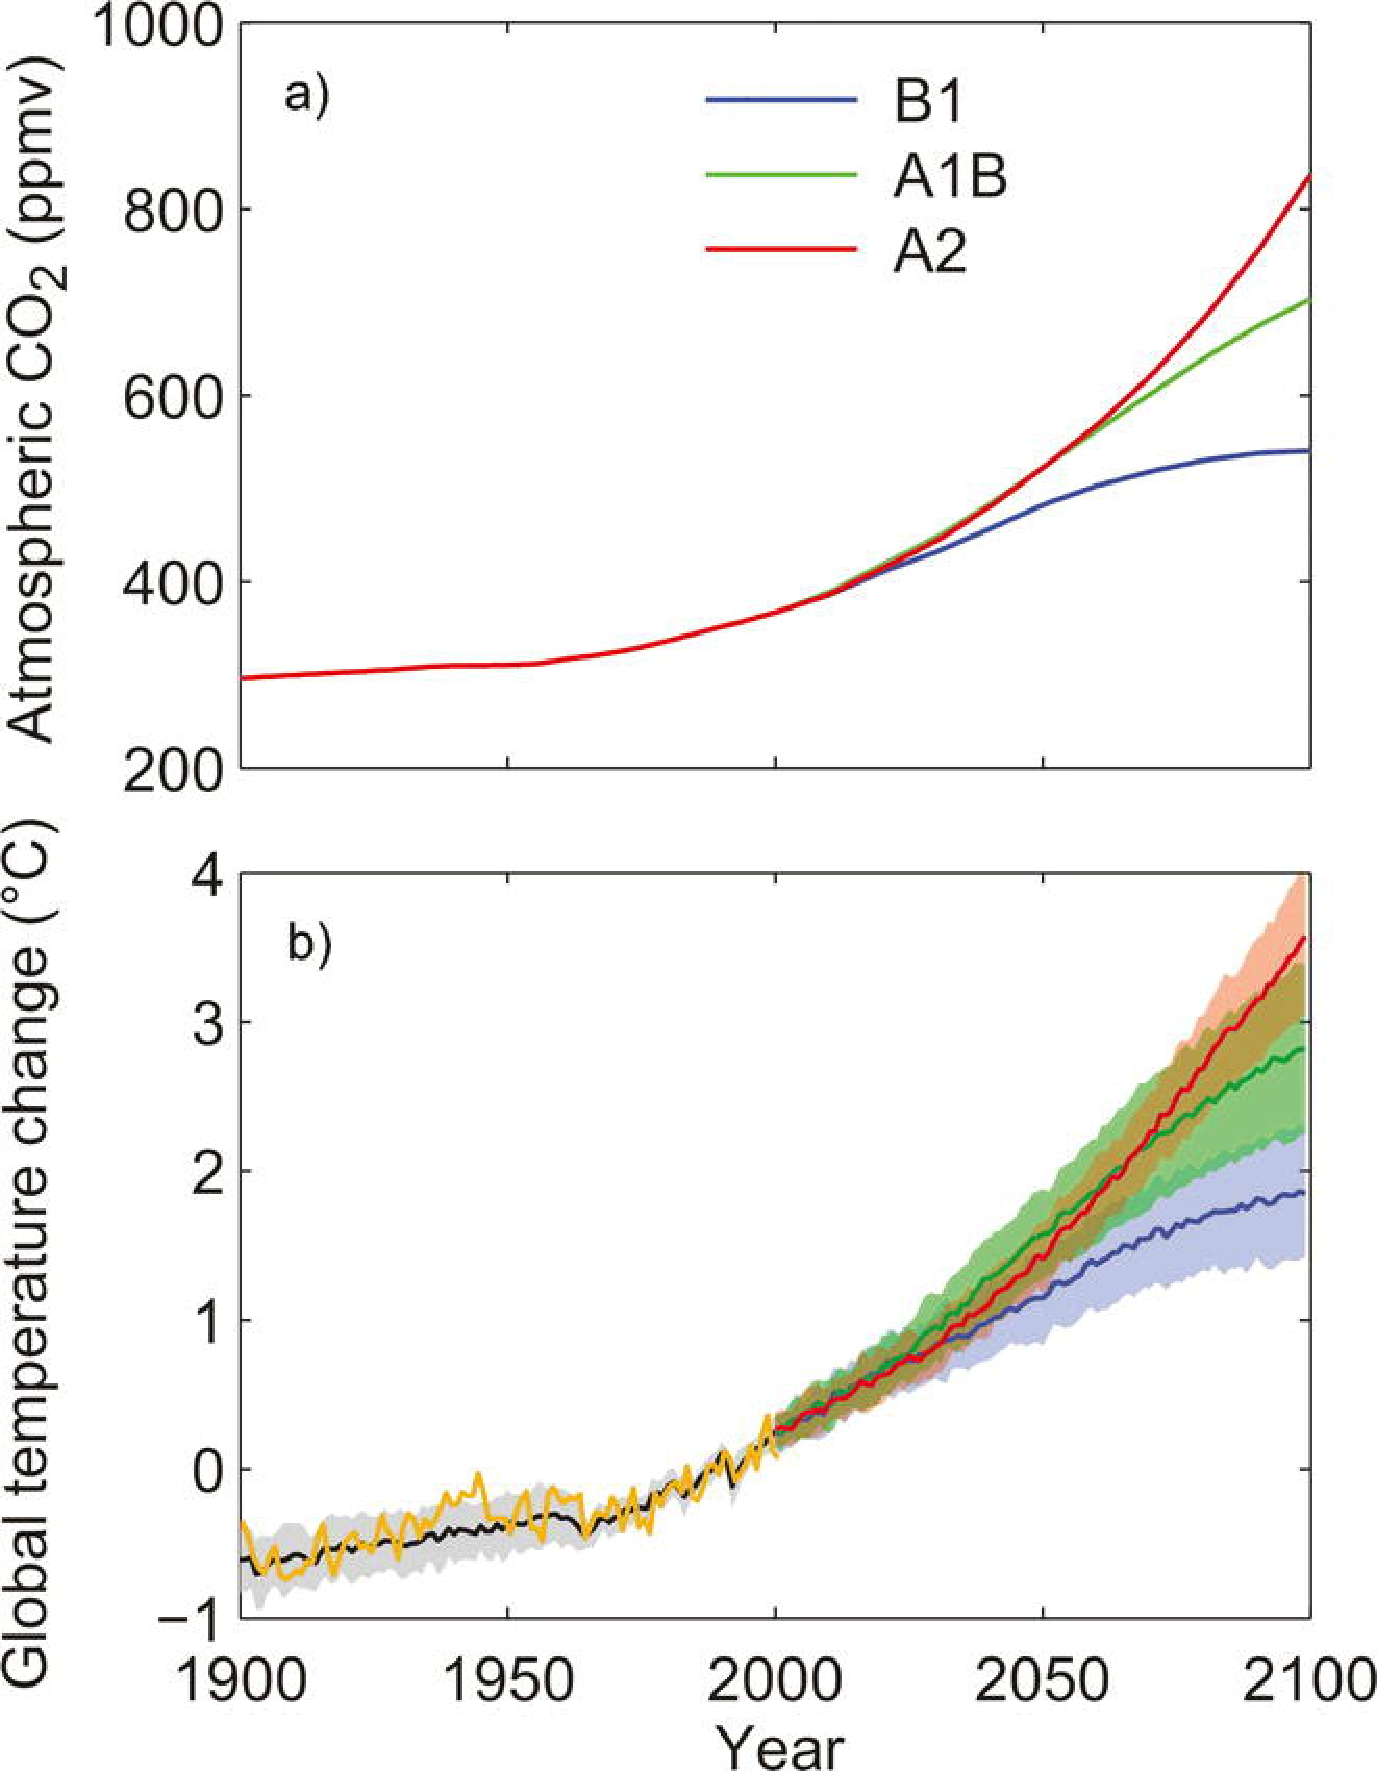
\includegraphics[width=19pc,angle=0]{figure01.pdf}\\
%  \caption{Enter the caption for your figure here.  Repeat as
%  necessary for each of your figures. Figure from \protect\cite{Knutti2008}.}\label{f1}
%\end{figure}

\begin{figure}[t]
\centering
\noindent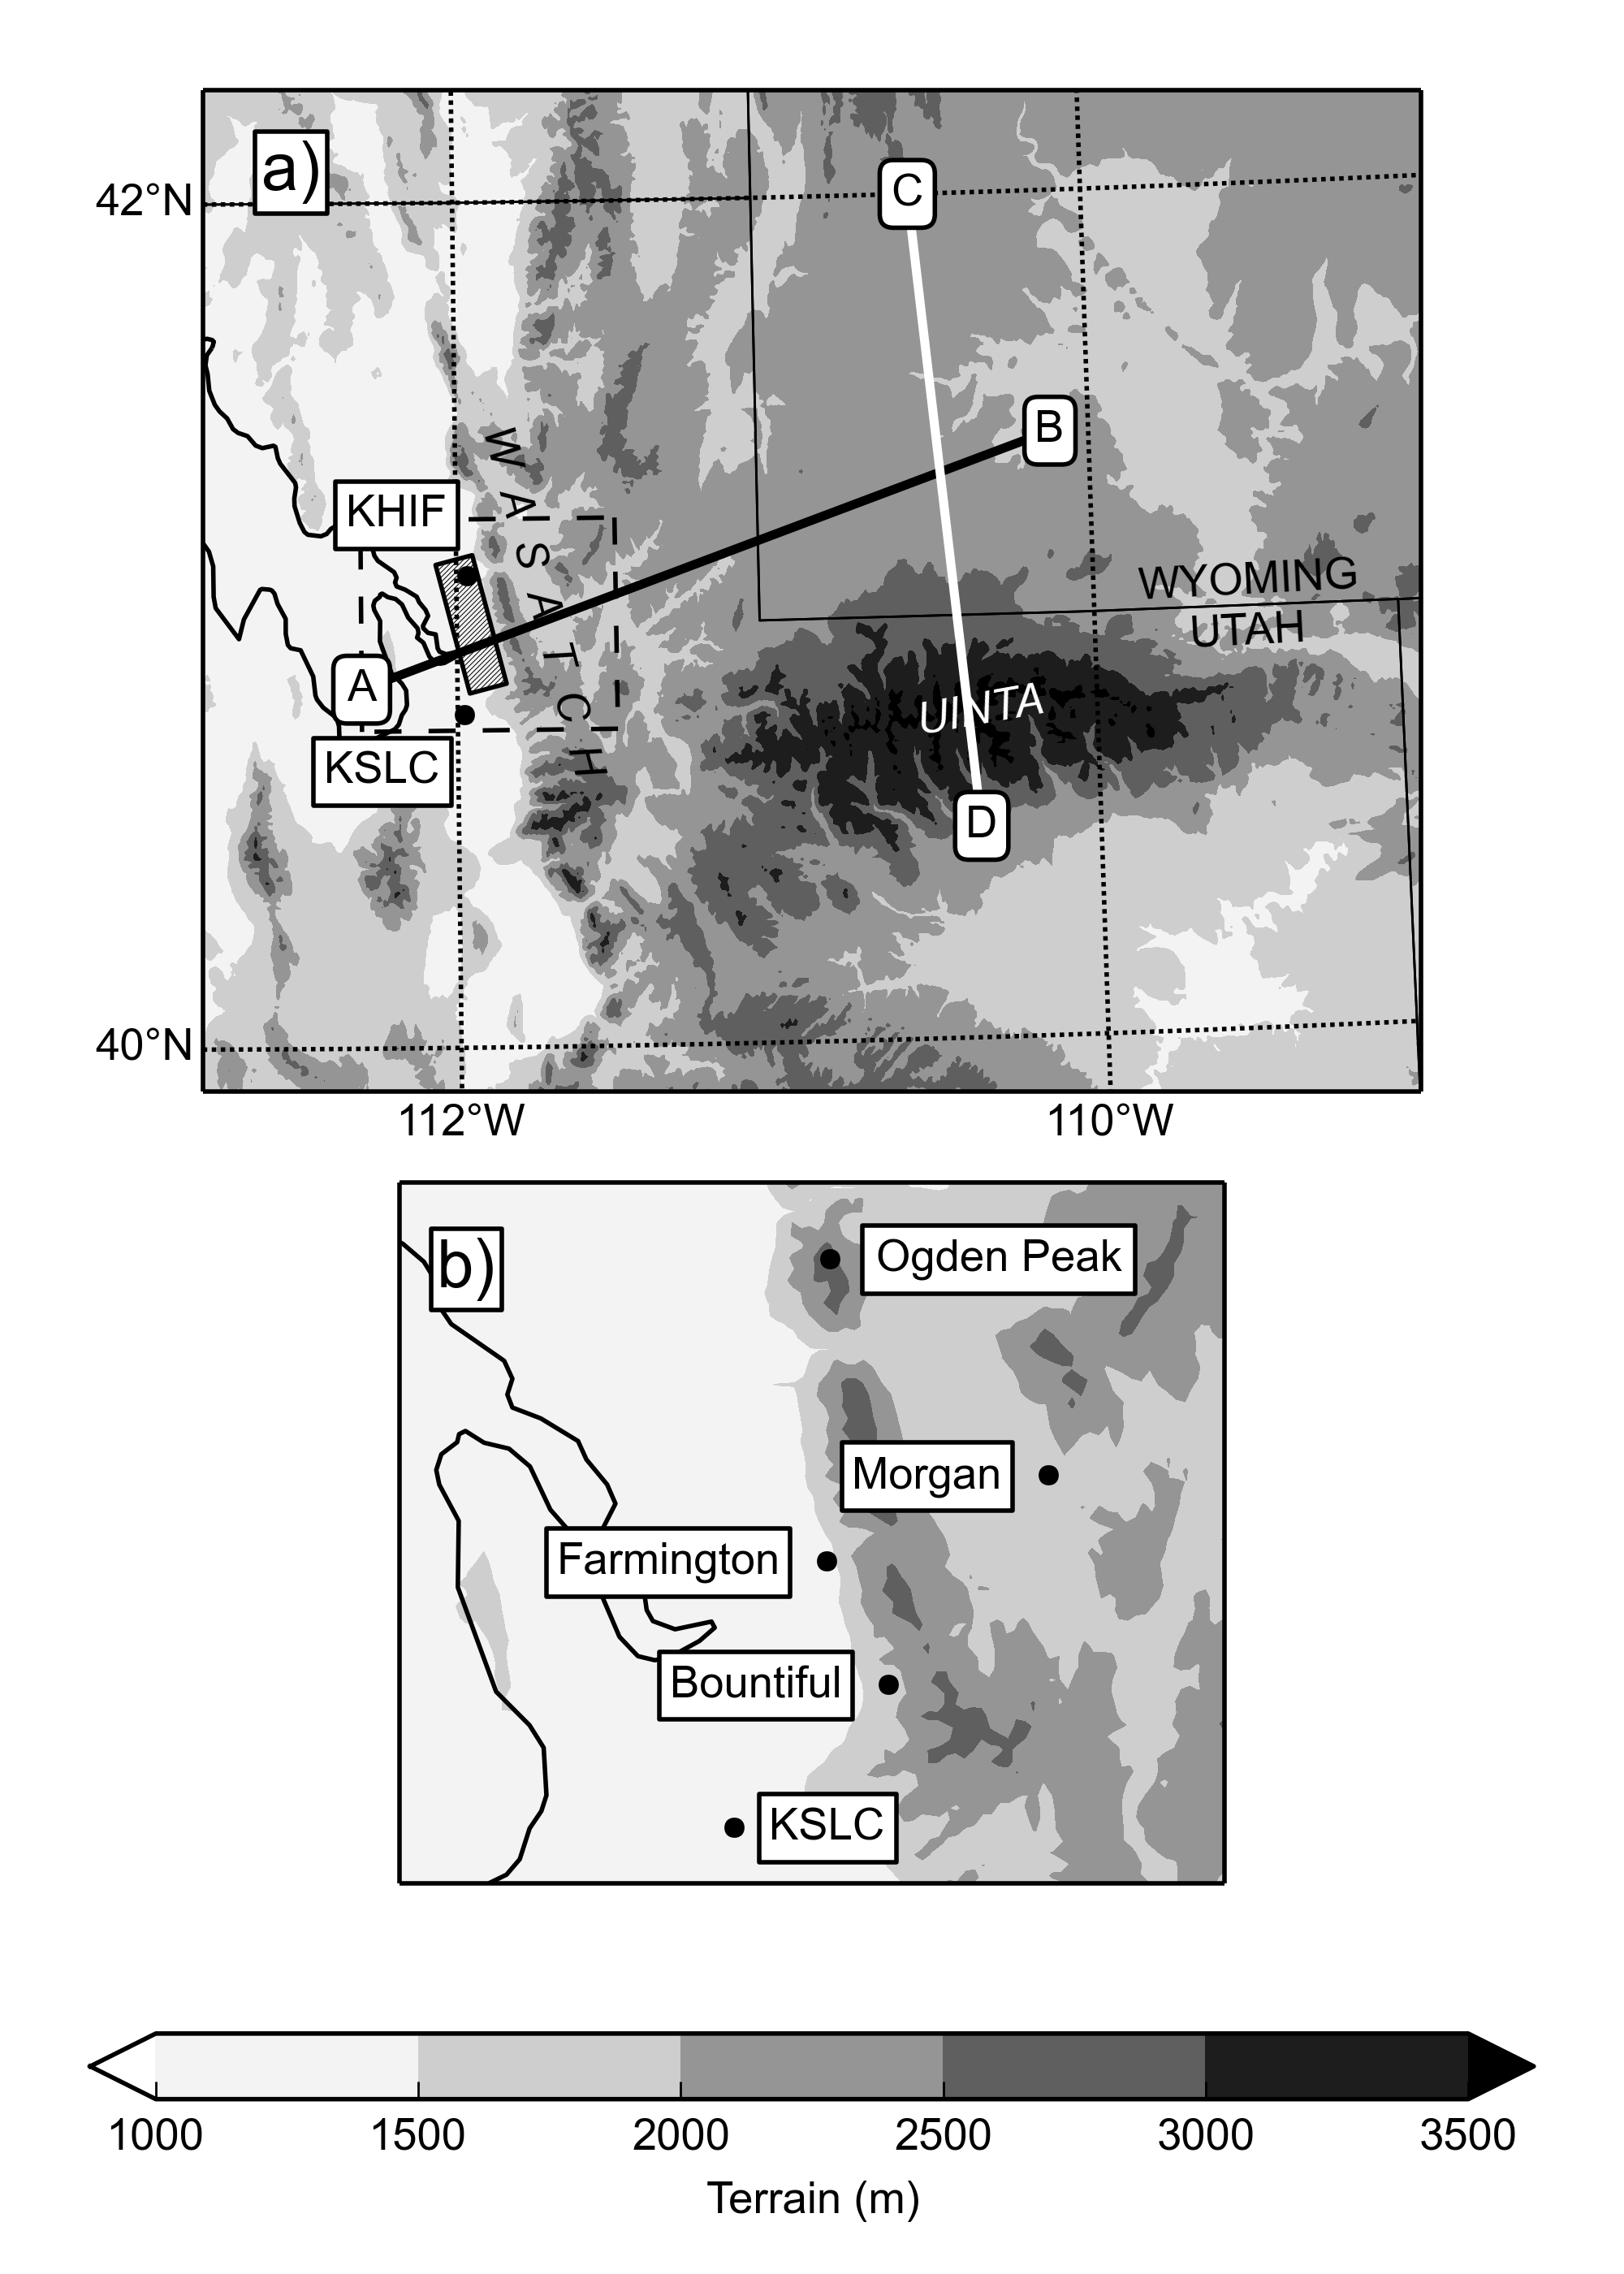
\includegraphics[width=0.77\textwidth]{map2}\\
\caption{Terrain elevation and locations in northern Utah and western Wyoming (shading). (a) Locations (Salt Lake International Airport, KSLC; and Hill Air Force Base, KHIF), mountain ranges, and cross-section paths mentioned in the text are shown.  The shaded rectangular box along the Wasatch Front approximately delineates the damage swath on 1 December 2011. The Wasatch Front is the low-lying region paralleling the west slopes of the Wasatch Mountains. (b) Zoomed-in view with locations discussed in the text.}
\label{fig:wasatchmap}
\end{figure}

\begin{figure}[t]
\centering
\noindent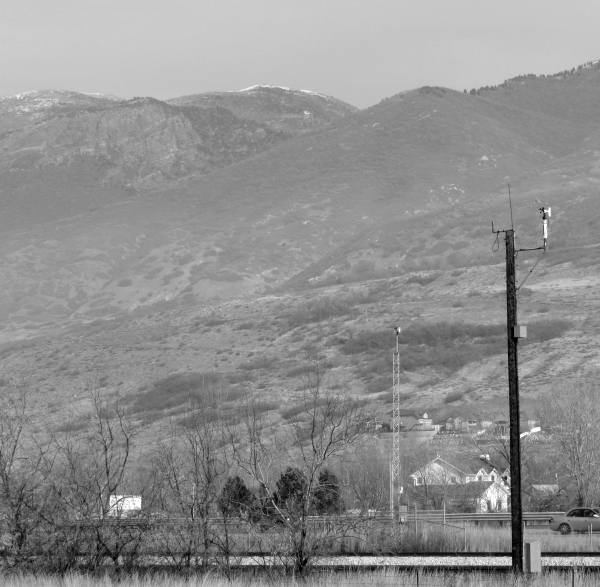
\includegraphics[width=0.7\textwidth]{cen_cenwws_small_crop_BW}\\
\caption{Anemometers installed in Centerville, UT, by Union Pacific Railroad (\MW{} identifier: UP028; foreground) and Utah Department of Transportation (CEN; background), at the location of strongest observed winds during the 1~December~2011 windstorm.}
\label{fig:cenwws}
\end{figure}

\begin{figure}[t]
\centering
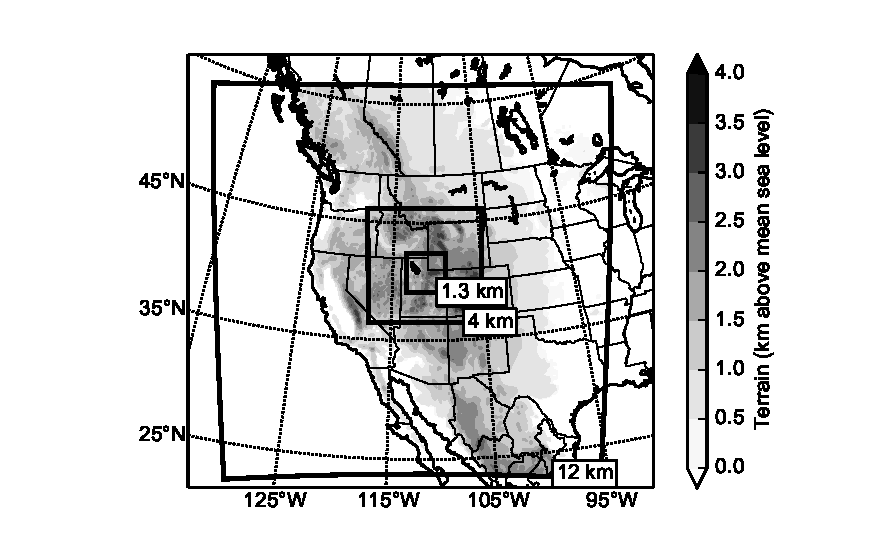
\includegraphics[width=0.9\textwidth,angle=0]{domains.pdf}\\
\caption{Domain areas for the 12-, 4-, and 1.3-km domains in the Weather Research and Forecasting model. Terrain is from the 12-km domain at 10-min resolution.}
\label{fig:domains}
\end{figure}

\begin{figure}[t]
\centering
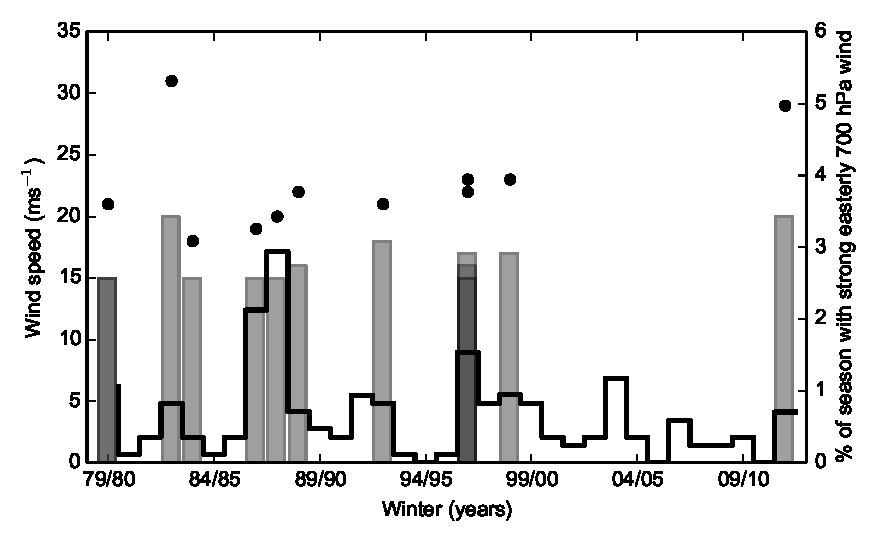
\includegraphics[width=0.9\textwidth]{climoplot.pdf}\\
\caption{Sustained wind (shaded bars) associated with downslope windstorms as a function of winter season at KHIF according to the scale on left. Filled circles indicate the maximum gust associated with each windstorm. Percent of season with strong (10\,\mps{}) 700-hPa winds from easterly direction in ERA-Interim Reanalysis data marked by black line according to scale on the right. Two (three) events occur in the winter of 1979/80 (1996/97) and hence overlap on the chart.}
\label{fig:climoplot}
\end{figure}

\begin{figure}[t]
\centering
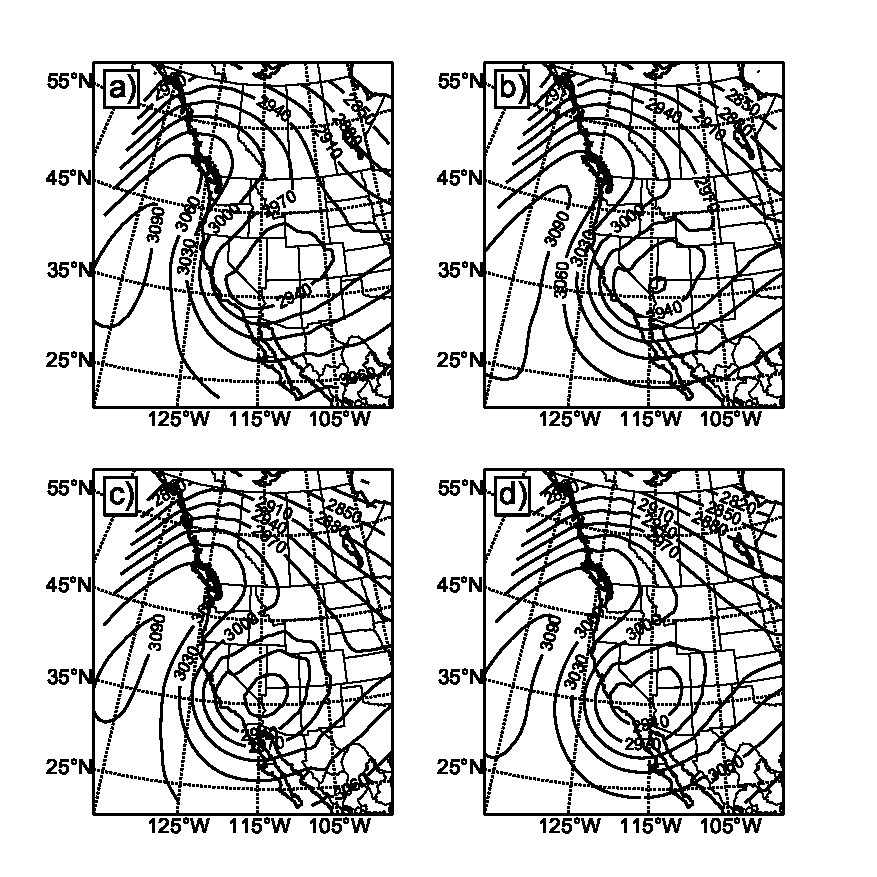
\includegraphics[width=0.9\textwidth]{composite_700hPa_Z.pdf}\\
\caption{Evolution of ERA-Interim 700-hPa geopotential height (contoured at 30-m intervals), composited over 13 downslope windstorm events at (a) 0000 UTC, (b) 0600 UTC, (c) 1200 UTC, and (d) 1800 UTC.}
\label{fig:700comp}
\end{figure}

\begin{figure}[t]
\centering
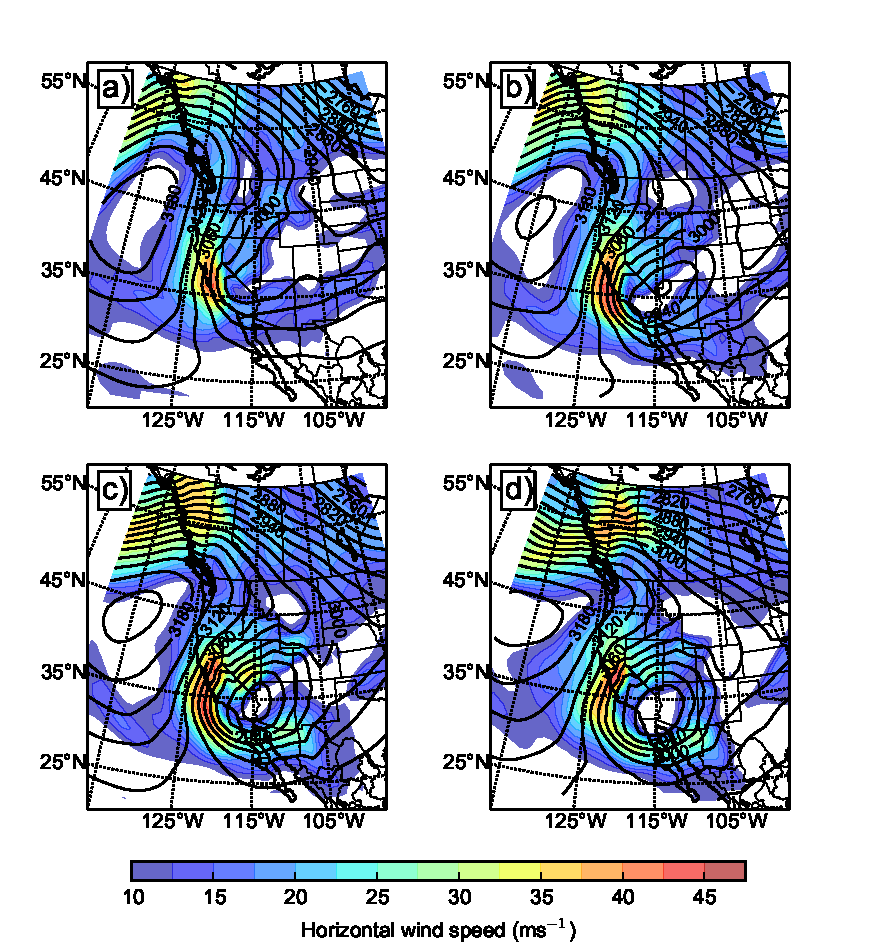
\includegraphics[width=0.9\textwidth]{dec1_Z_wind_ERA.pdf}\\
\caption{Evolution of 700-hPa geopotential height (contoured at 30-m intervals) and wind speed (shading according to scale) on 1 December 2011, taken from the ERA-Interim dataset, at (a) 0000 UTC, (b) 0600 UTC, (c) 1200 UTC, and (d) 1800 UTC.}
\label{fig:geopot4panel}
\end{figure}

%\begin{sidewaysfigure}
%\centering
%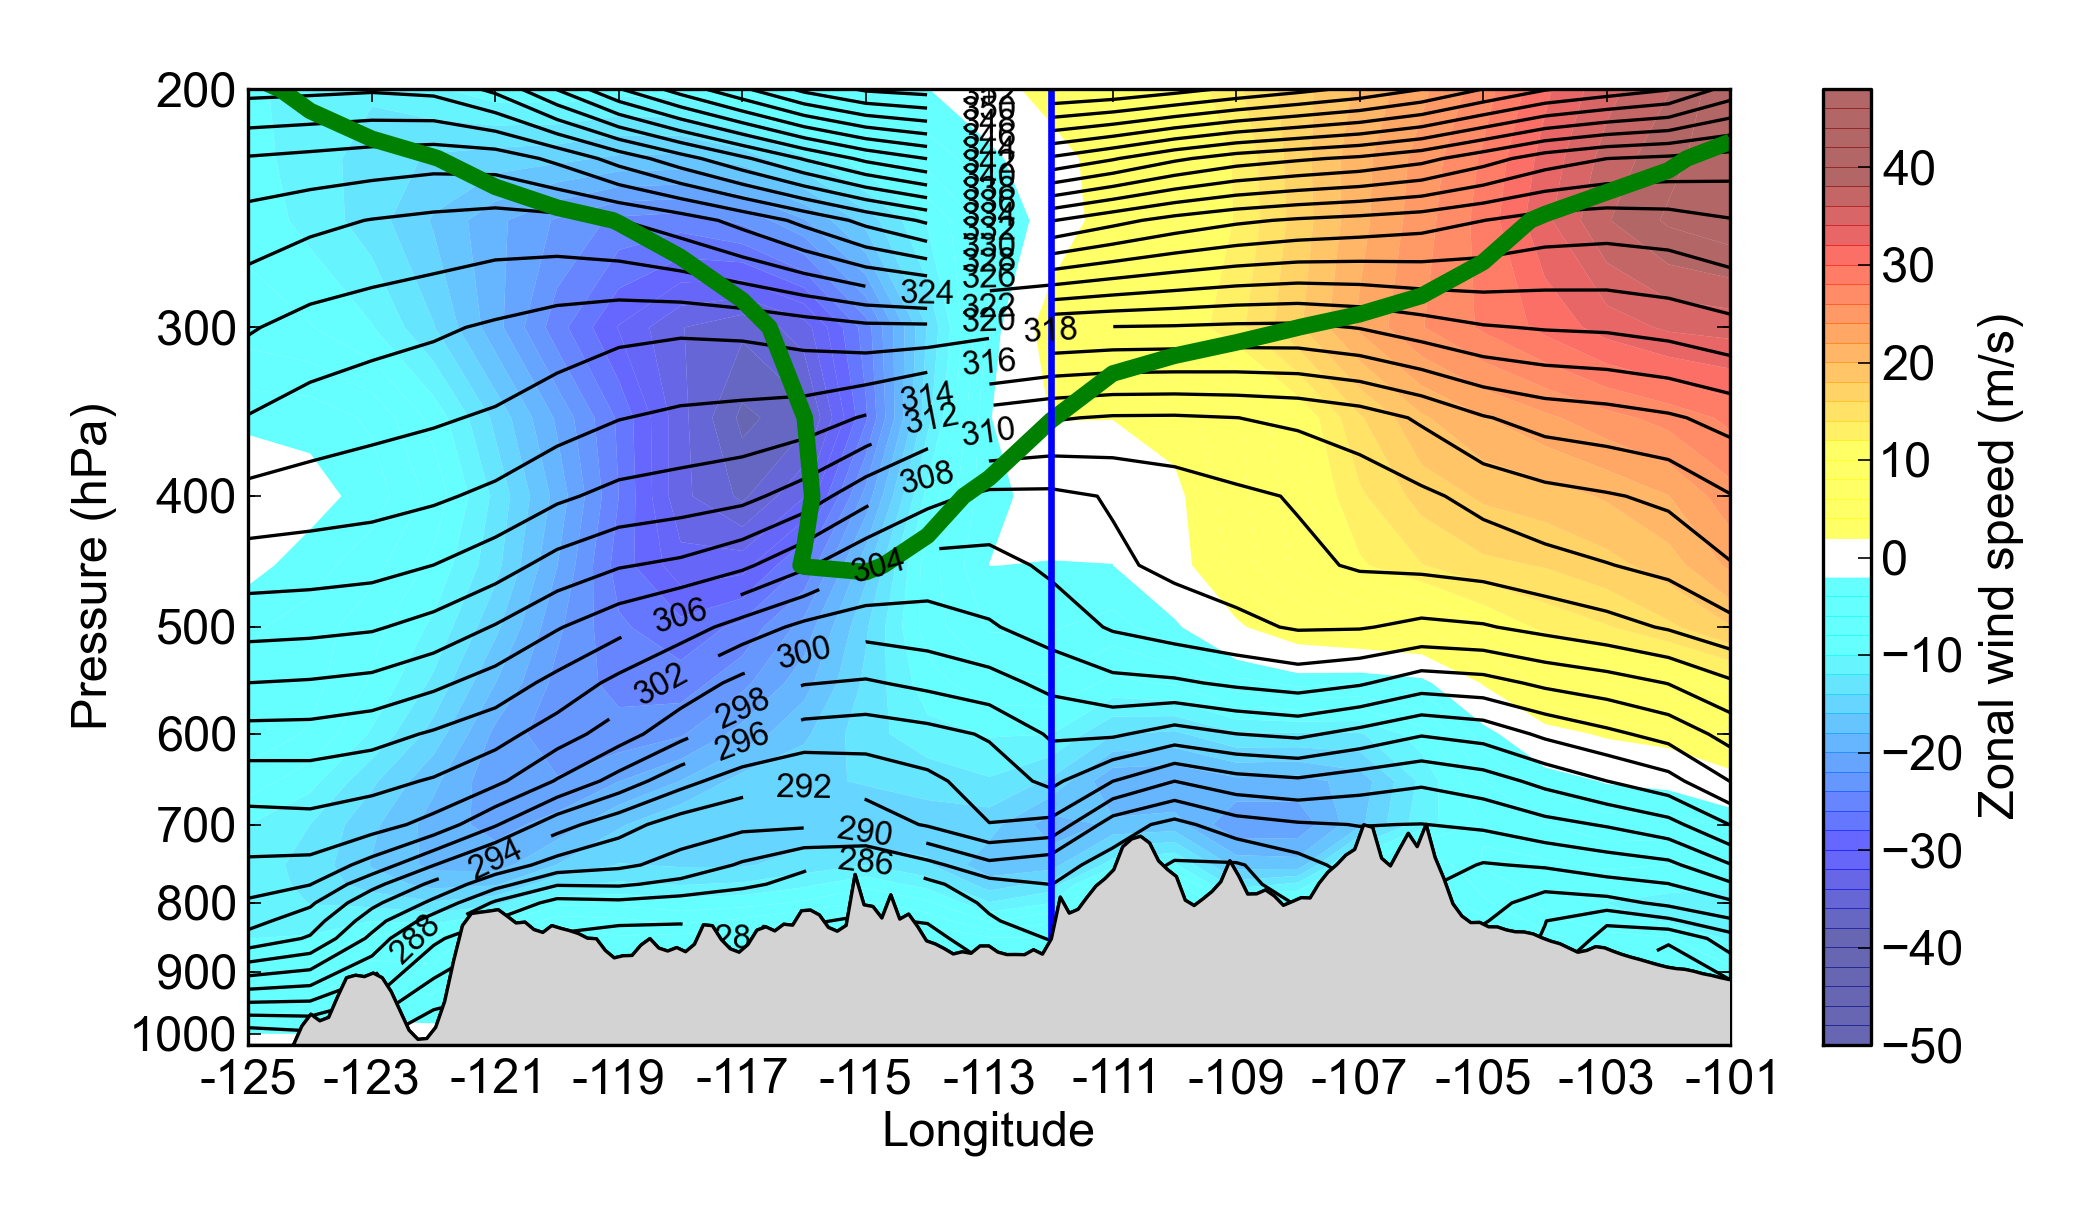
\includegraphics[width=54pc,angle=0]{cross_section_12z}\\
%\caption{West--east cross-section of ERA-Interim reanalysis potential temperature (contoured at 2-K intervals) and zonal wind (shading according to the scale on the right) at 1200\,UTC 1 December 2011. Cross-section path is marked by red lines in Fig. \ref{fig:geopot4panel}. Green contour denotes height of dynamic tropopause (i.e., where potential vorticity $=$ 2\,PVU). Blue vertical line denotes the location of the Wasatch Front.}
%\label{fig:eraxs}
%\end{figure}
%\end{sidewaysfigure}




\begin{figure}[t]
\centering
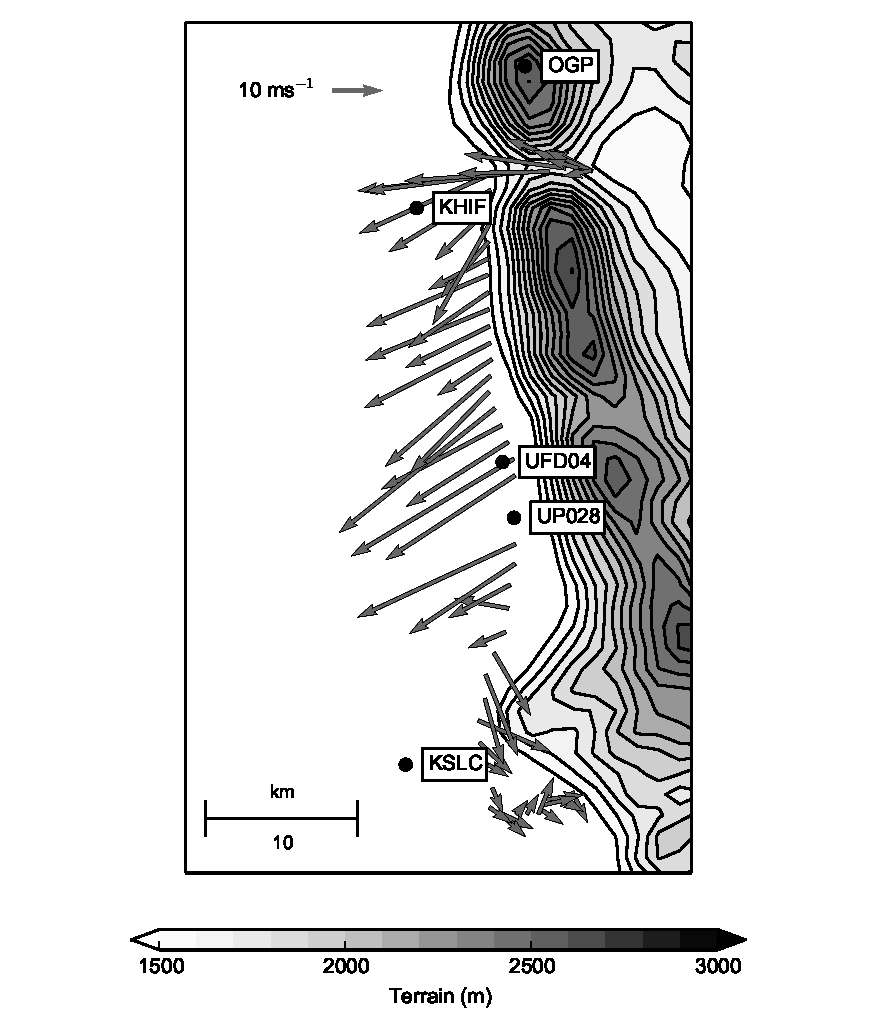
\includegraphics[width=0.9\textwidth]{mobmes_09.pdf}\\
\caption{Mobile wind observations from 0915--1015\,UTC. Vector arrows are relative to scale in top-left. Distance is according to the scale in bottom-left. Filled contours indicate terrain, taken from innermost WRF domain, with scale at bottom. Observation stations mentioned in text are labeled.}
\label{fig:mobmes}
\end{figure}

\begin{figure}[t]
\centering
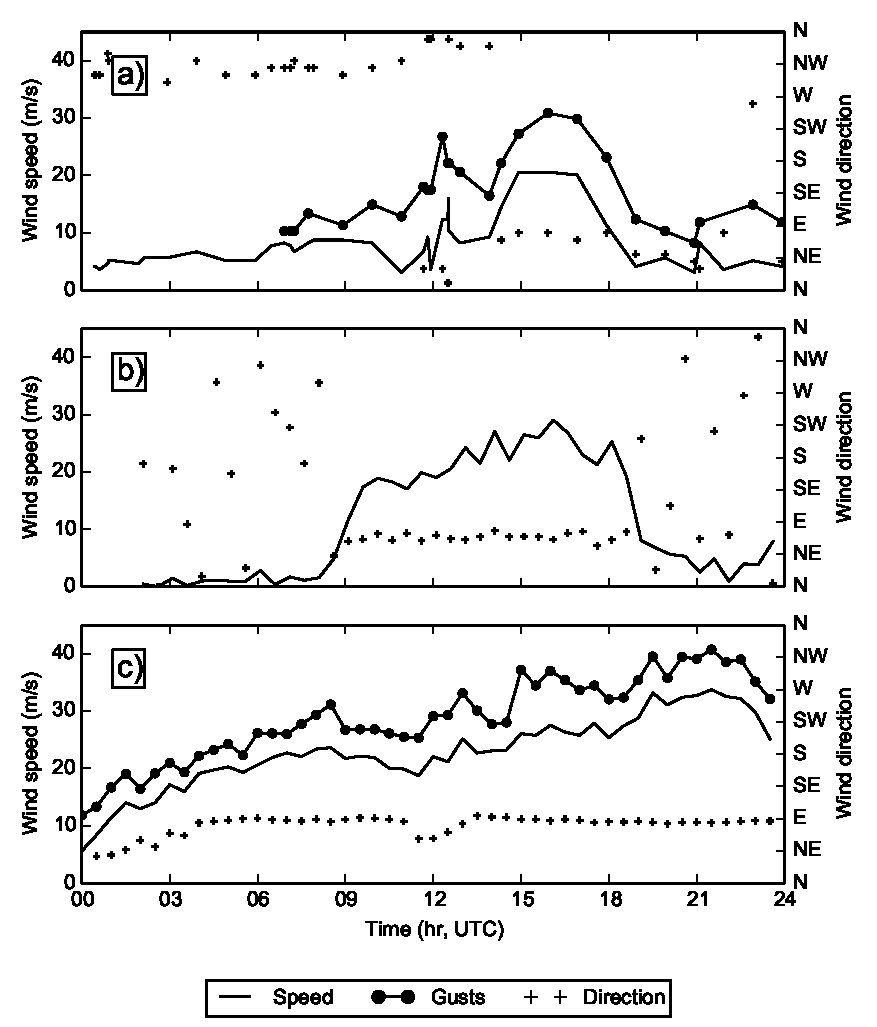
\includegraphics[width=0.9\textwidth]{obs_comp.pdf}\\
\caption{Surface wind observations at (a) KHIF, (b) UFD04, and (c) OGP on 1 December 2011. Wind speed, wind gust, and wind direction shown by solid lines, filled circles, and crosses, respectively. All available KHIF observations are shown; for clarity, UFD04 and OGP data are sampled at 30-min intervals from the data available at higher reporting intervals.}
\label{fig:ob_ts}
\end{figure}

%\begin{sidewaysfigure}
%\centering
%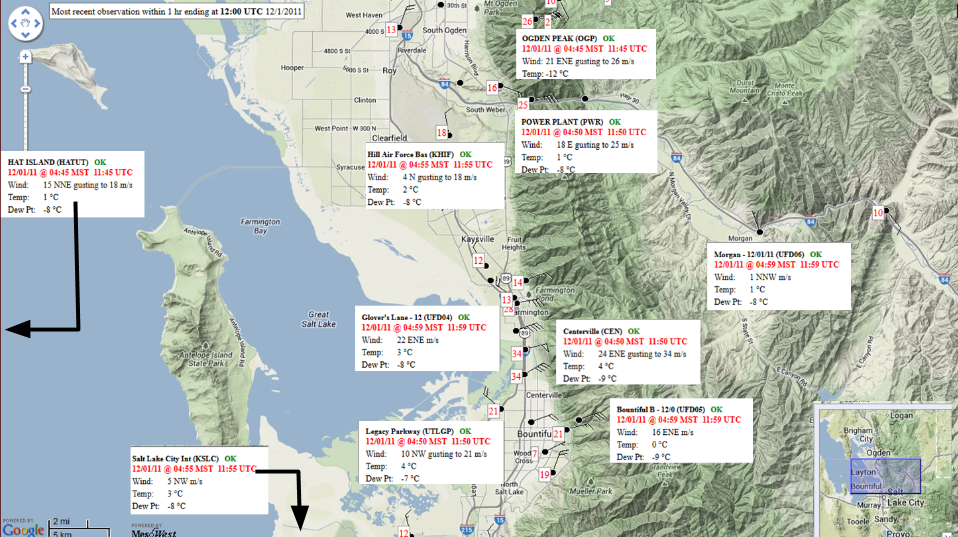
\includegraphics[width=0.8\textwidth]{MesoWest12zAnno}\\
%\caption{Surface observations in northern Utah at 1200\,UTC 1 December 2011. Wind speed denoted by barbs (full barb 5 \mps) and wind gusts in \mps{} labeled where available. Wind, temperature, and dewpoint temperature shown for selected stations.}
%\label{fig:mesowest12z}
%\end{sidewaysfigure}

%\begin{figure}[t]
%\centering
%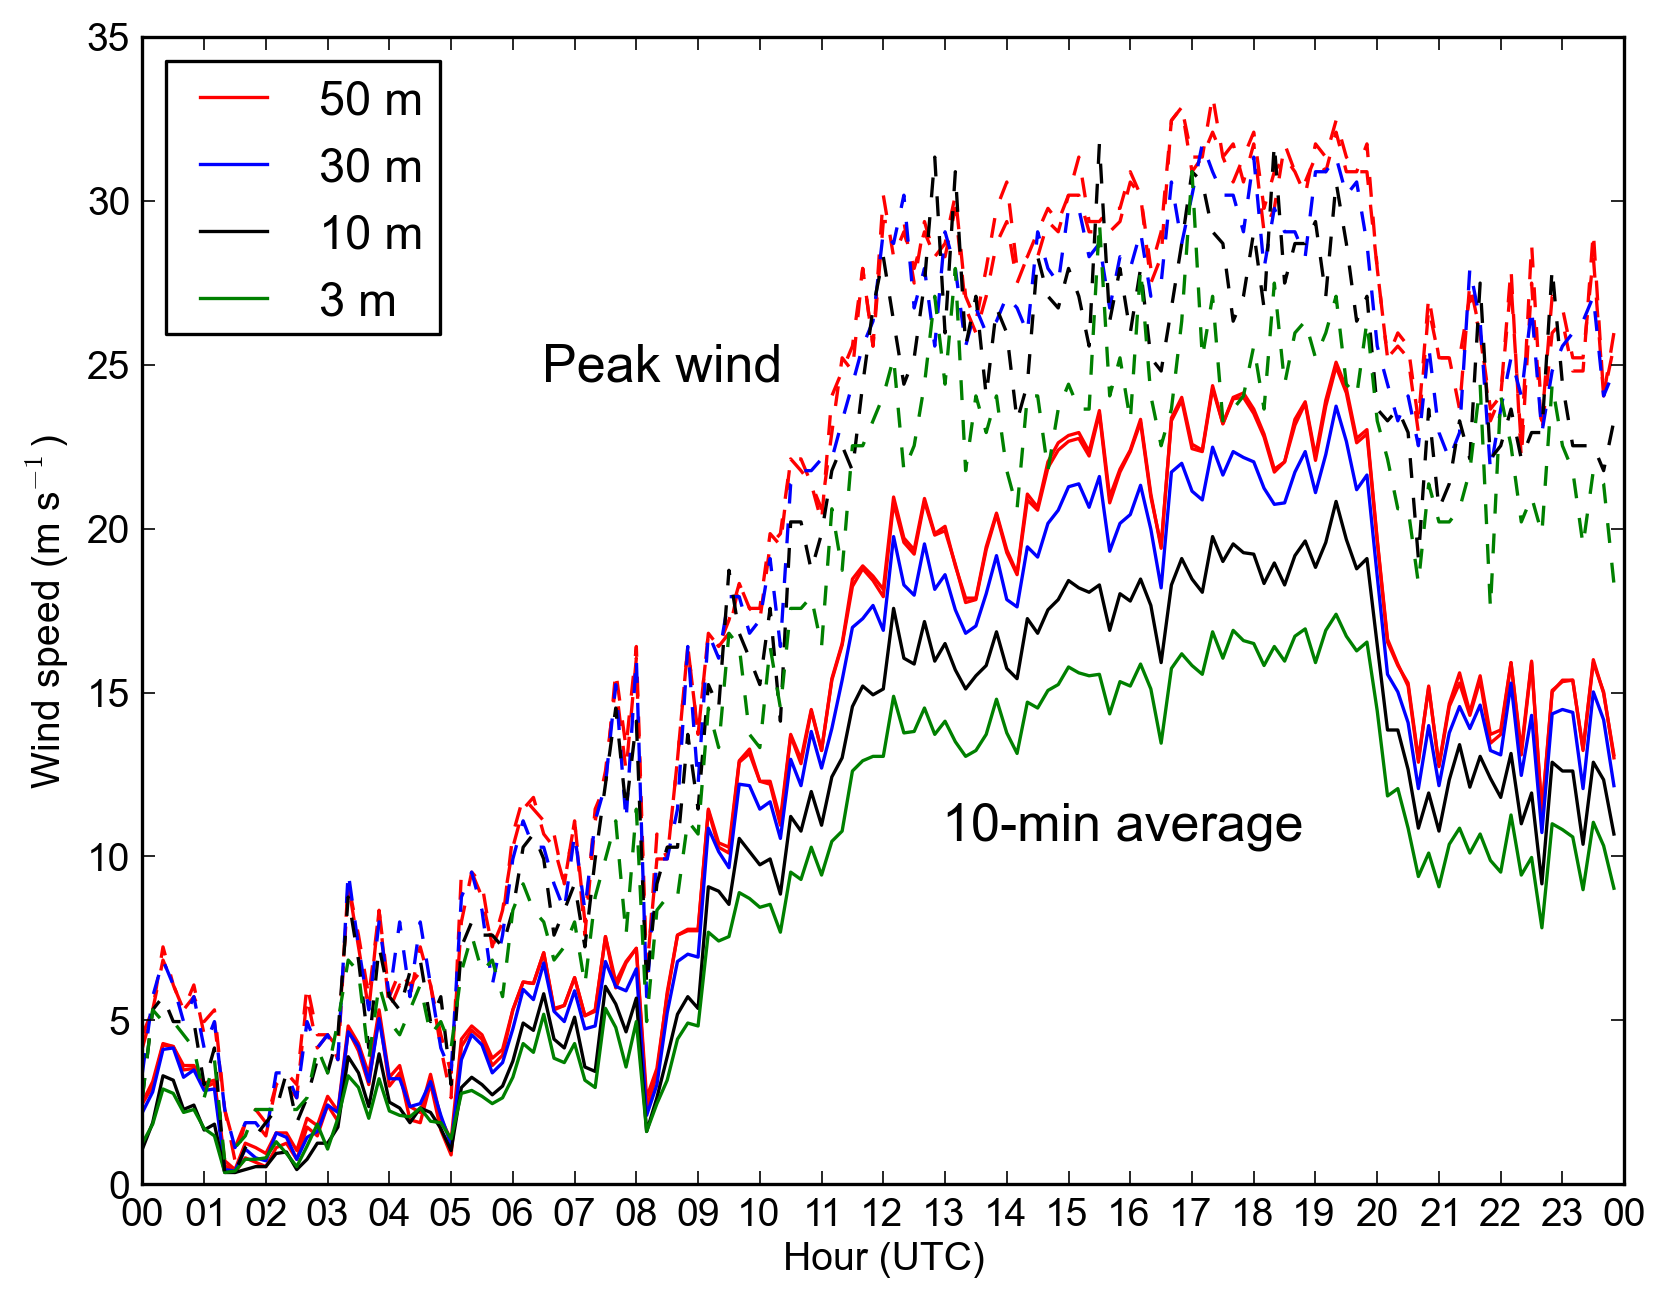
\includegraphics[width=39pc,angle=0]{towerdata}\\
%\caption{50-m tower observations of wind speed as a function of sensor elevation above ground level at the mouth of Weber Canyon, 1~December 2011.}
%\label{fig:tower}
%\end{figure}

\begin{figure}[t]
\centering
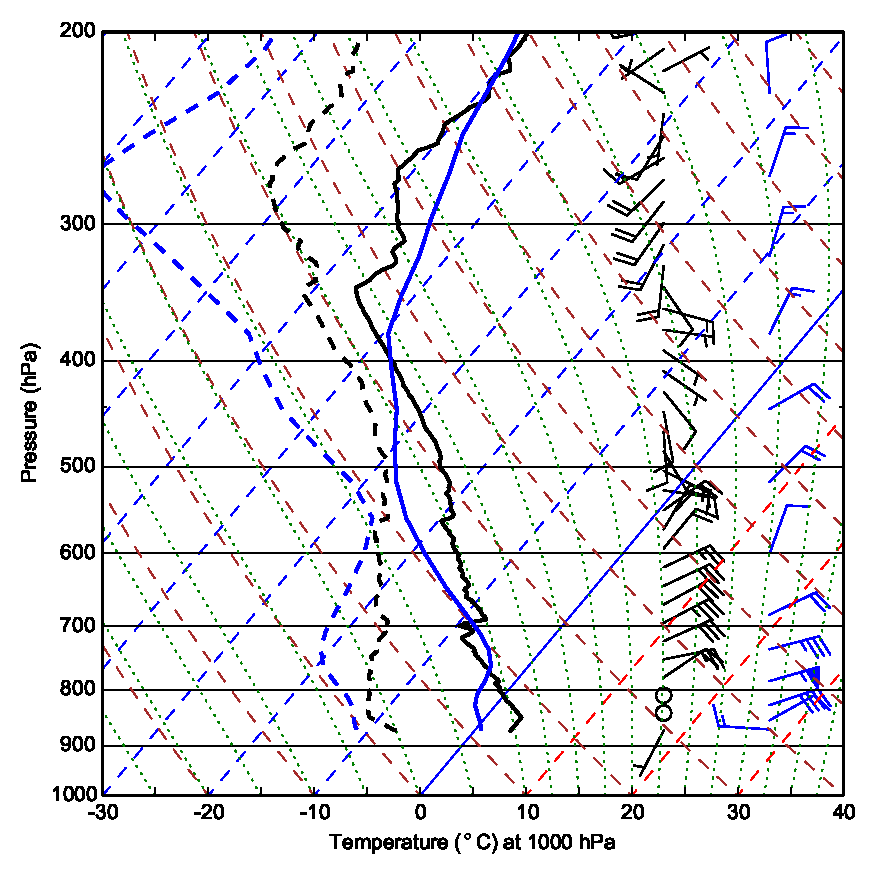
\includegraphics[width=0.9\textwidth]{KSLC_SkewT.pdf}
\caption{Skew-T log-P profiles at 1200\,UTC 1 December 2011, from observed rawinsonde launch at KSLC (black lines) and from the WRF Control simulation at the nearest grid point (blue lines). Temperature, dew-point temperature, and wind denoted by solid lines, dashed lines, and barbs (full barb 5 \mps), respectively. For clarity, wind barbs from only selected model levels are shown.}
\label{fig:kslcWRF}
\end{figure}

\begin{figure}[t]
\centering
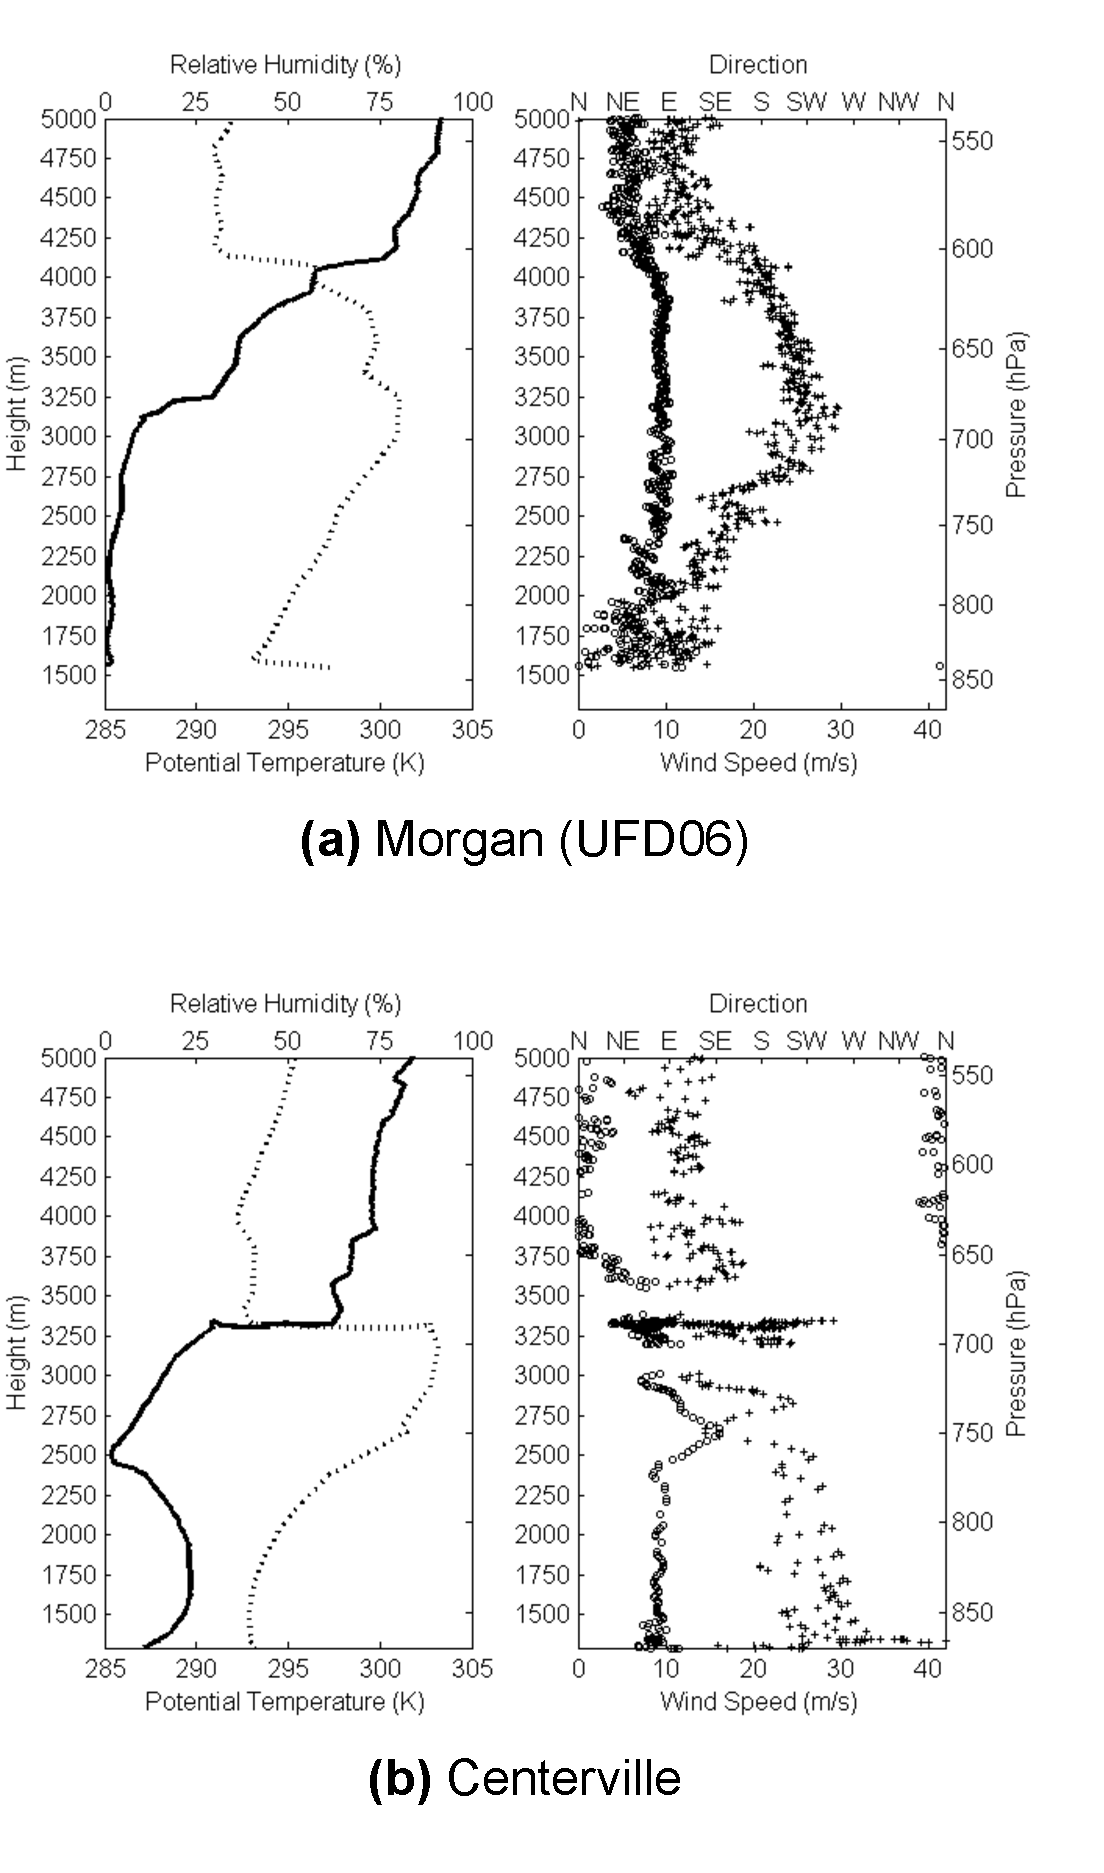
\includegraphics[width=27pc,angle=0]{sound_comp}
\caption{Vertical profiles of observed rawinsonde data near Morgan, UT, and Centerville, UT (near UP028). (a) Potential temperature (solid line), relative humidity (dashed line), wind speed (crosses), and wind direction (open circles) at Morgan, UT, at 1800\,UTC 1 December 2011, as a function of height. (b) As in (a) but for the 1200\,UTC Centerville, UT launch.}
\label{fig:sound}
\end{figure}

\begin{figure}[t]
\centering
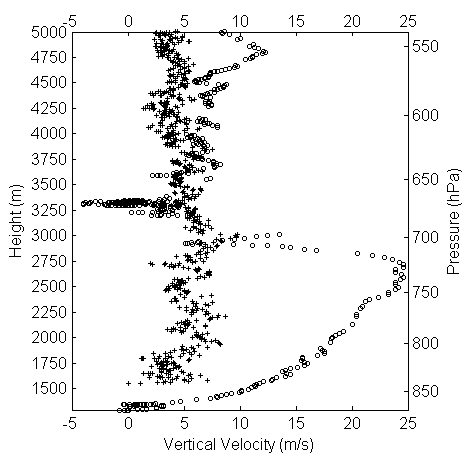
\includegraphics[width=21pc,angle=0]{vertical_vel_crop}
\caption{Comparison of rawinsonde ascent rates (\mps) at Morgan, UT (1800\,UTC; crosses) and Centerville (1200\,UTC; open circles).}
\label{fig:ascent}
\end{figure}

\begin{figure}[t]
\centering
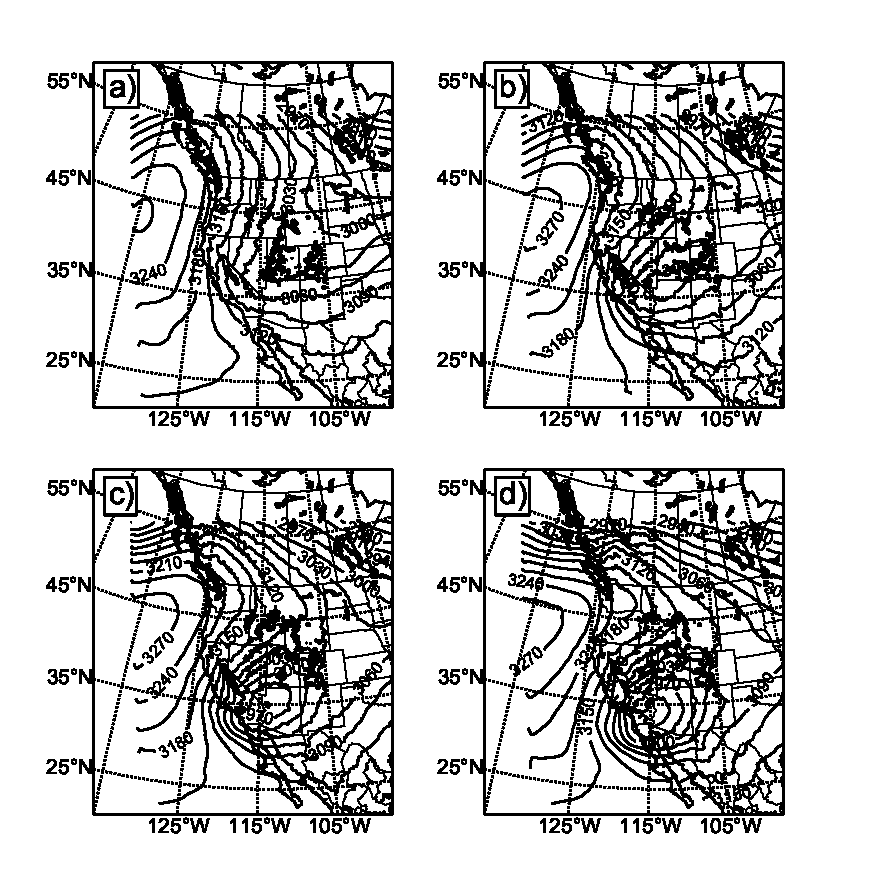
\includegraphics[width=0.9\textwidth]{WRF700.pdf}
\caption{WRF Control simulation 700-hPa geopotential height fields (contoured at 30-m interval), at (a) 0000 UTC, (b) 0600 UTC, (c) 1200 UTC, and (d) 1800 UTC, all 1 December 2011. Noisy contours result from the 700-hPa surface intersecting the model terrain.}
\label{fig:NAM-C_700}
\end{figure}

\begin{figure}[t]
\centering
\includegraphics[width=0.9\textwidth]{verification.pdf}
\caption{Comparison of observed surface wind speeds (colored circles) versus Control-simulation surface wind speeds (shading), both according to scale at bottom. The wind measurements are taken from the observation time closest to (a) 1200\,UTC and (b) 2100\,UTC, within 30\,min either side of the respective times, for each available station. WRF innermost-domain terrain contoured every 400\,m for reference; Antelope Island marked with ``AI".}
\label{fig:verif}
\end{figure}

%\begin{sidewaysfigure}
\begin{figure}[p]
\centering
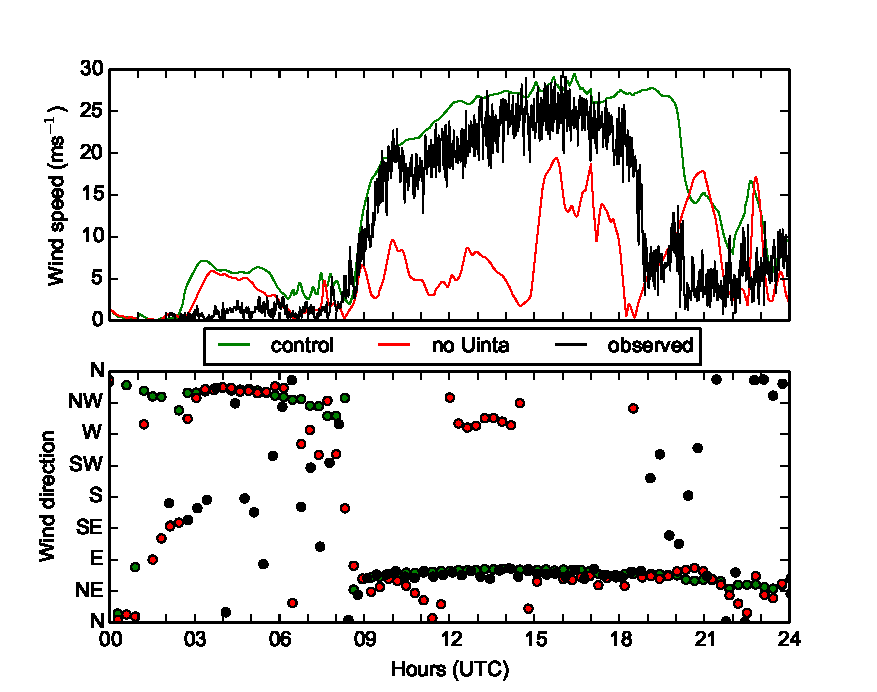
\includegraphics[width=0.9\textwidth]{GloversLane_ts}
\caption{Observed and simulated surface winds at Farmington (UFD04), UT on 1 December 2011. Observed wind speeds and wind directions from UFD04 are denoted by black solid lines and filled circles, respectively. Simulated surface wind speeds and directions from the Control (No-Uinta) simulations are shown by the green (red) solid lines and filled circles, respectively. Wind direction data from all three sources have been subsampled to every 20 minutes for clarity.}
\label{fig:glove_ts}
\end{figure}
%\end{sidewaysfigure}

\begin{figure}[t]
   \centering
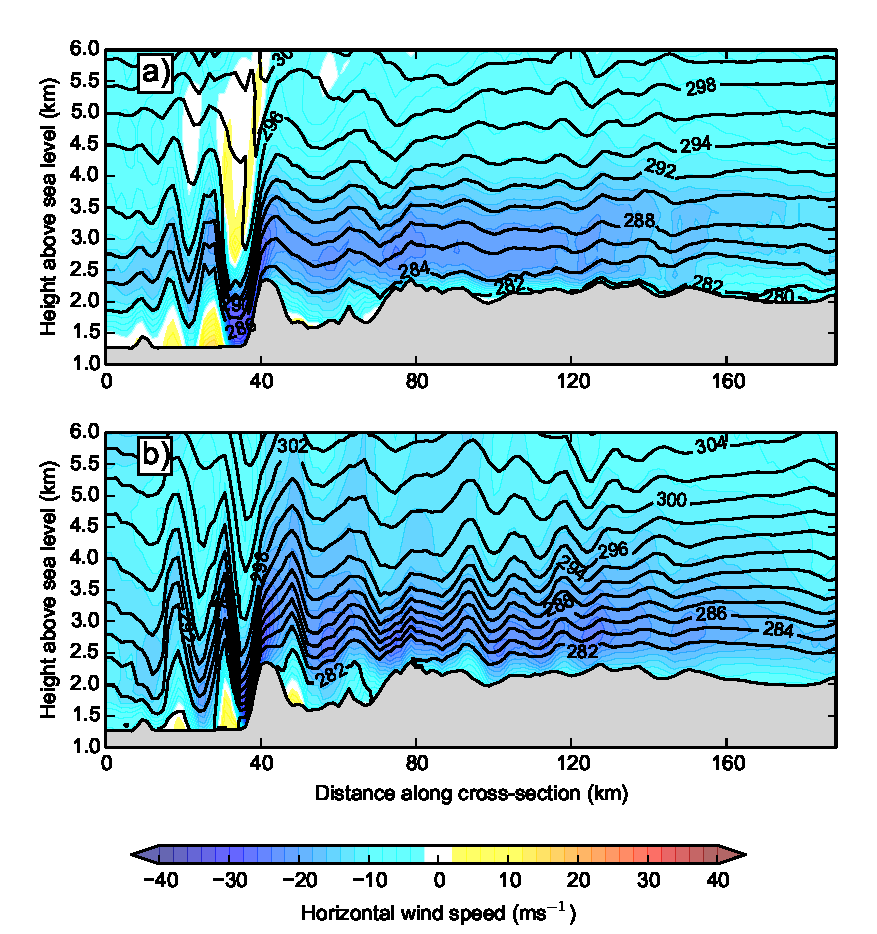
\includegraphics[width=0.9\textwidth]{yes_xs_westeast_parawind.pdf}
   \caption{Perpendicular-to-Wasatch cross-section from innermost WRF domain (A--B in Fig.~\ref{fig:wasatchmap}) at (a) 1200\,UTC and (b) 2100\,UTC, 1 December 2011. Shading denotes plane-parallel wind component according to the scale (e.g., blue indicates flow from right to left), while potential temperature is contoured at an interval of 2\,K.}
   \label{fig:ppxswu}
\end{figure}

\begin{figure}[t]
   \centering
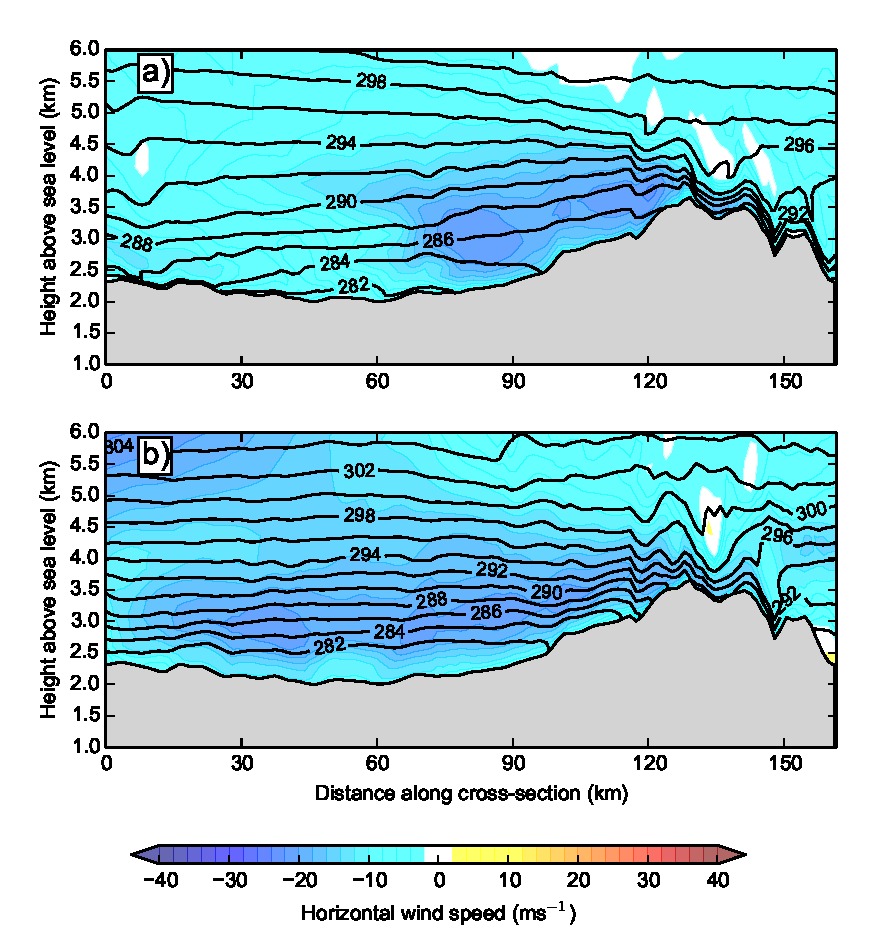
\includegraphics[width=0.9\textwidth]{yes_xs_northsouth_perpwind.pdf}
   \caption{Roughly north--south cross-section from innermost WRF domain (C--D in Fig.~\ref{fig:wasatchmap}) through west-central Wyoming (left) to the southern slopes of the Uintas (right) at (a) 1200\,UTC and (b) 2100\,UTC, 1 December 2011. Shading denotes wind component in and out of the page (e.g., blue indicates predominantly easterly flow out of the page) according to the scale; potential temperature is contoured at an interval of 2\,K.}
   \label{fig:normxswu}
\end{figure}

\begin{figure}[t]
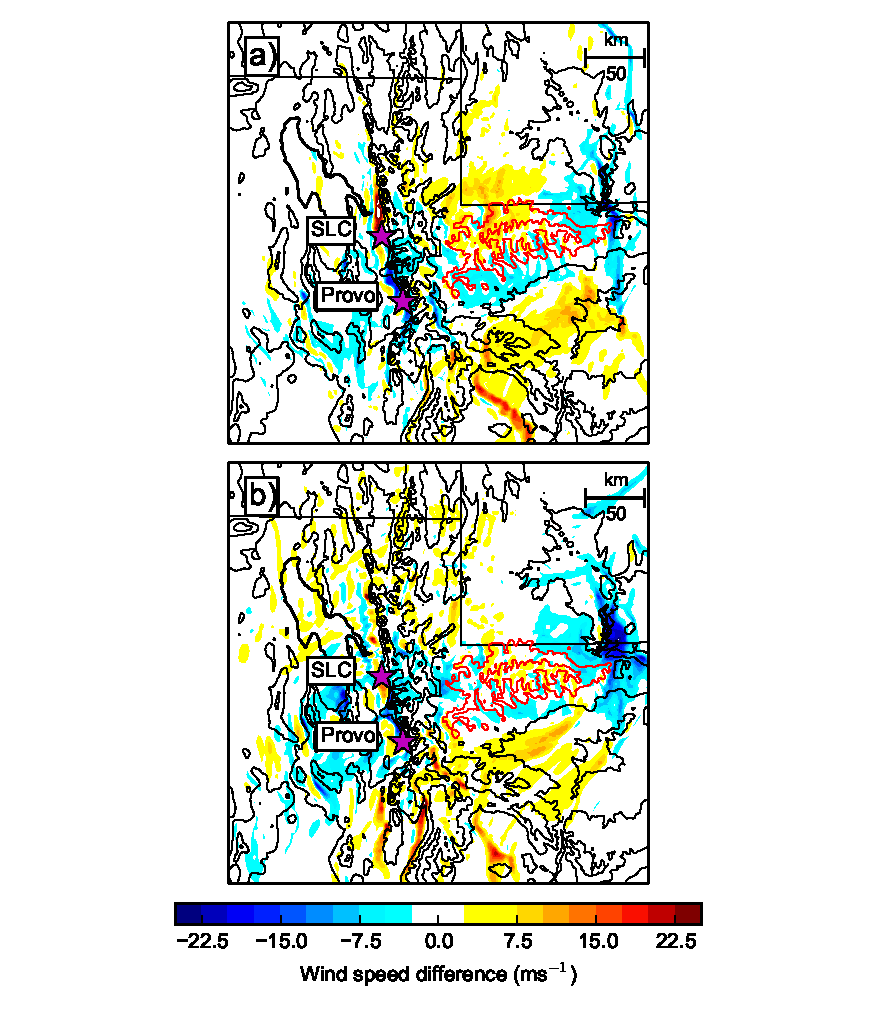
\includegraphics[width=0.9\textwidth]{eastdiff.pdf}
   \caption{Zonal wind difference (No-Uinta minus Control), shaded according to the scale at the bottom, at (a) 1200\,UTC and (b) 2100\,UTC, 1 December 2011. Black (red) contours at 500-m intervals denote the elevation of the terrain used in both the Control and No-Uinta (Control only) simulations. Blue (red) indicates an increase (decrease) in easterly wind in this location as a result of removing the Uinta mountains.}
   \label{fig:eastdiff}
\end{figure}

\begin{figure}[p]
   \centering
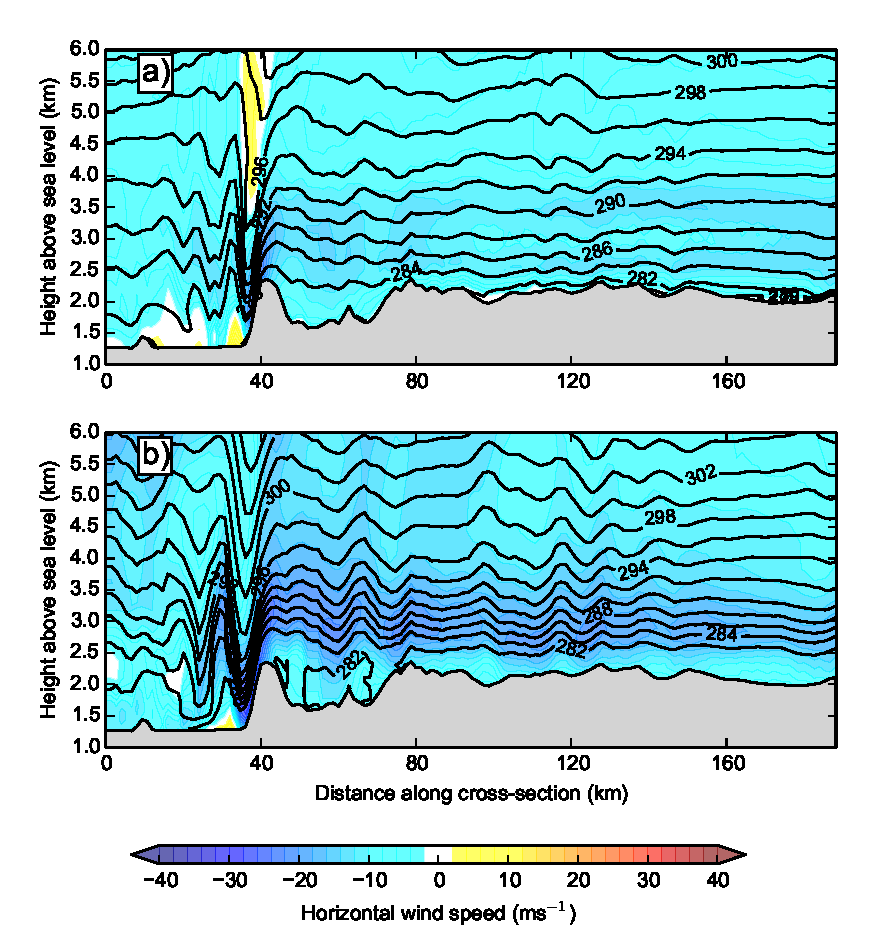
\includegraphics[width=0.9\textwidth]{no_xs_westeast_parawind.pdf}
   \caption{As in Fig.~\ref{fig:ppxswu}, but from the no-Uinta WRF simulation.}
   \label{fig:ppxsnu}
\end{figure}

\begin{figure}[p]
   \centering
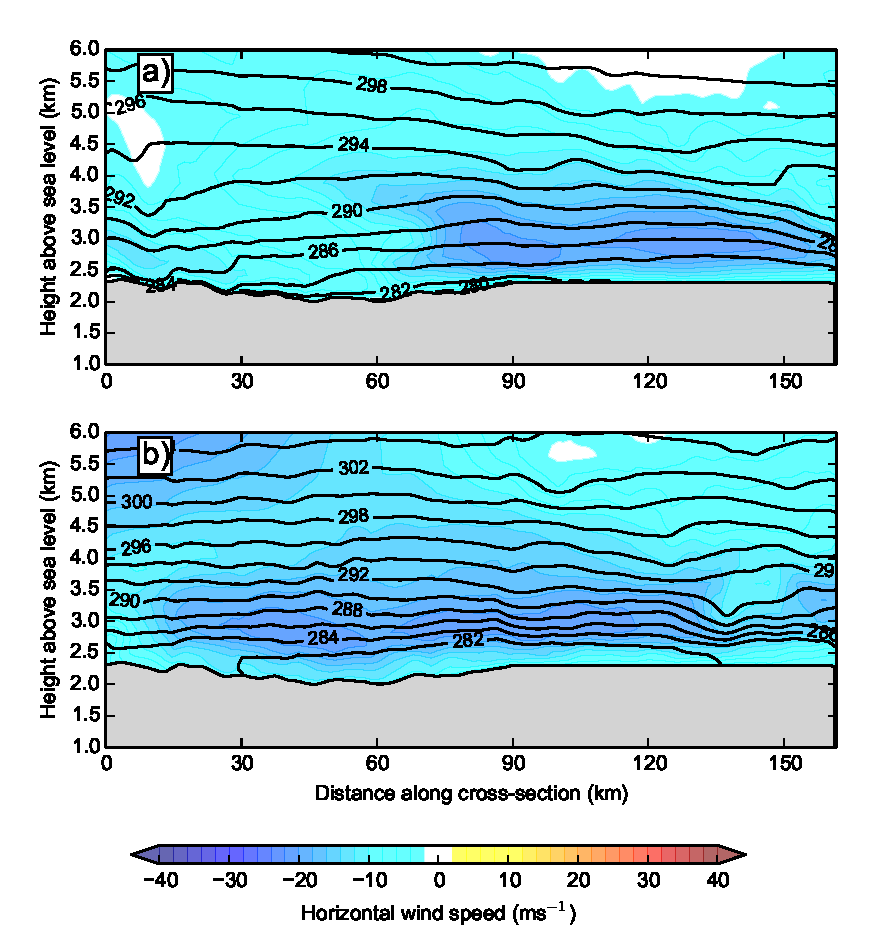
\includegraphics[width=0.9\textwidth]{no_xs_northsouth_perpwind.pdf}
   \caption{As in Fig.~\ref{fig:normxswu}, but from the no-Uinta WRF simulation.}
   \label{fig:normxsnu}
\end{figure}

%%%%%%%%%%%%%%%%%%%%%%%%%%%%%%%%%%%%%%%%%%%%%%%%%%%%%%%%%%%%%%%%%%%%%
% TABLES
%%%%%%%%%%%%%%%%%%%%%%%%%%%%%%%%%%%%%%%%%%%%%%%%%%%%%%%%%%%%%%%%%%%%%
%\begin{table}[t]
%\caption{This is a sample table caption and table layout.  Enter as many tables as
%  necessary at the end of your manuscript. Table from Lorenz (1963).}\label{t1}
%\begin{center}
%\begin{tabular}{ccccrrcrc}
%\hline\hline
%$N$ & $X$ & $Y$ & $Z$\\
%\hline
% 0000 & 0000 & 0010 & 0000 \\
% 0005 & 0004 & 0012 & 0000 \\
% 0010 & 0009 & 0020 & 0000 \\
% 0015 & 0016 & 0036 & 0002 \\
% 0020 & 0030 & 0066 & 0007 \\
% 0025 & 0054 & 0115 & 0024 \\
%\hline
%\end{tabular}
%\end{center}
%\end{table}

%\begin{sidewaystable}[t]
%\caption{Approximate characteristic linear slopes upstream of some documented downslope-windstorm locations. }
%\label{tab:slope}
%\begin{center}
%\begin{tabular}{ccccc}
%\hline \hline 
%\textbf{Location} & \textbf{Crest--base} & \textbf{Crest--base}& \textbf{Slope} & \textbf{Reference} \\
%& \textbf{horiz. distance} & \textbf{vertical distance}& & \\ \hline
%{\textbf{Wasatch Front, UT, USA}} & 5.9\,km & 1.3\,km & 22\% & \citet{Horel2002a} \\ 
%{\textbf{(Wasatch Front in WRF)}} & (6.5\,km) & (1.1\,km) & (17\%) & (30-s WRF terrain) \\ 
%{\textbf{Owens Valley, CA, USA}} & 11\,km & 2.5\,km & 22\% & \citet{Grubisic2008} \\ 
%{\textbf{High Point, NJ, USA}} & 1.2\,km & 0.2\,km & 19\% & \citet{Decker2011} \\ 
%{\textbf{Juneau, AK, USA}} & 7.4\,km & 1.1\,km & 15\% & \citet{Colman1992} \\ 
%{\textbf{East Falkland, Falkland Is.}} & 3.3\,km & 0.4\,km & 13\% & \citet{Mobbs2005} \\ 
%{\textbf{Senj, Croatia}} & 8.7\,km & 1.0\,km & 11\% & \citet{Smith1987} \\ 
%{\textbf{Helm Wind, UK}} & 5.3\,km & 0.6\,km & 11\% & \citet{Manley1945} \\ 
%{\textbf{Boulder, CO, USA}} & 39\,km & 2.3\,km & 6\% & \citet{Lilly1972} \\ 
%{\textbf{Mendoza, Argentina}} & 116\,km & 5.0\,km & 2\% & \citet{Norte2008} \\ 
%\hline
%\end{tabular}
%\end{center}
%\end{sidewaystable}


\begin{table}[t]
\caption{Parameterization schemes used in numerical modeling configuration.}
\label{tab:param}
\begin{center}
\begin{tabular}{cc}
\hline \hline
{\textbf{Parameterization}} & {\textbf{Scheme}} \\ \hline
{\textbf{Microphysics}} & WRF Single-Moment 3-class Scheme  \\ 
{\textbf{Longwave Radiation}} & RRTM Scheme  \\ 
{\textbf{Shortwave Radiation}} & Dudhia Scheme \\ 
{\textbf{Surface Layer}} & MM5 Similarity \\ 
{\textbf{Land Surface}} & Noah Land Surface Model (with snow effect) \\ 
{\textbf{Urban Surface}} & Switched off  \\ 
{\textbf{Planetary Boundary Layer}} & Yonsei University Scheme  \\ 
{\textbf{Cumulus Parameterization}} & Kain-Fritsch Scheme (12-km, 4-km domains only)  \\ 
{\textbf{Latent/Sensible Heat Flux}} & Allowed \\ 
{\textbf{Vertical Velocity Damping}} & Switched off  \\ 
{\textbf{6th Order Horizontal Diffusion}} & Simple (12-km domain only) \\ \hline
\end{tabular}
\end{center}
\end{table}

\begin{table}[t]
\caption{Downslope windstorm events at KHIF as defined by this study.}
\label{tab:dsws}
\begin{center}
\begin{tabular}{cccc}
\hline \hline   
\textbf{Date} & \textbf{Time of} & \textbf{Max.~wind speed} & \textbf{Max.~wind gust} \\
& \textbf{max.~wind, UTC} & \textbf{\mps{} (mph)} & \textbf{\mps{} (mph)} \\ \hline
{9 October 1979} & 1500 & 15 (34) & 21 (48) \\ 
{19 January 1980} & 1200 & 15 (34) & 22 (49) \\ 
{4 April 1983} & 1700 & 21 (46) & 31 (70) \\ 
{30 March 1984} & 1200 & 15 (34) & 18 (41) \\ 
{16 January 1987} & 1740 & 15 (34) & 20 (44) \\ 
{24 December 1987} & 0700 & 15 (34) & 21 (46) \\ 
{15 December 1988} & 1200 & 16 (36) & 23 (51) \\ 
{30 January 1993} & 1700 & 18 (41) & 21 (48) \\ 
{12 January 1997} & 1100 & 17 (38) & 23 (52) \\ 
{24 February 1997} & 1700 & 18 (40) & 23 (51) \\ 
{2 April 1997} & 1600 & 15 (34) & 24 (53) \\ 
{23 April 1999} & 1755 & 18 (40) & 24 (53) \\ 
{1 December 2011} & 1655 & 20 (45) & 30 (67) \\ 
\hline
\end{tabular}
\end{center}
\end{table}

%
\end{document}
